\documentclass[11pt,a4paper]{ctexart}
\usepackage{amsmath, amsthm, amssymb, graphicx,mathrsfs}
\usepackage{geometry}
\usepackage[colorlinks=true,hidelinks]{hyperref}
\geometry{left=1.24cm, right=1.24cm, top=1.91cm, bottom=1.91cm}
\title{经典控制理论}
\author{W·D·Gaster}

\renewcommand{\d}{{\rm d}}
\newcommand{\e}{{\rm e}}
\renewcommand{\j}{{\rm j}}
\newcommand{\mb}{\symbfit}

\usepackage{booktabs}
\usepackage{unicode-math}   % 添加\symbfit以实现加粗斜体命令
\usepackage{pifont}         %使用带圈数字序号
\usepackage{enumitem}       %自定义列表序号
\usepackage{subcaption}     %图片左右排列

\graphicspath{{figures/}} % 指定图片路径
\usepackage{float}

\makeatletter
\newcommand{\xleftrightarrow}[2][]{\ext@arrow 3359\leftrightarrowfill@{#1}{#2}}
\makeatother

\usepackage{wrapfig} % 文字包围图片

\begin{document}

\maketitle
\thispagestyle{empty}
\newpage

\tableofcontents
\thispagestyle{empty}
\newpage

\setcounter{page}{1}

\section{自动控制系统的基本概念}
    \subsection{控制系统的分类}
    按是否满足叠加性和齐次性分为：线性系统 or 非线性系统

    按参数是否随时间变化分为：定常（时不变）系统 or 时变系统（非线性系统：自治系统 or 非自治系统）

    按信号的连续性分为：连续系统 or 离散系统

    按输入输出的数目分为：单输入单输出系统（SISO） or 多输入多输出系统（MIMO）
    
    按是否存在反馈回路分为：开环控制系统 or 闭环控制系统
    \vspace{-10pt}
    \begin{figure}[H]
        \centering
        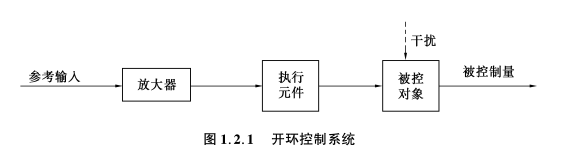
\includegraphics[width=8cm]{开环控制系统.png}
        \caption{开环控制系统结构框图}
    
        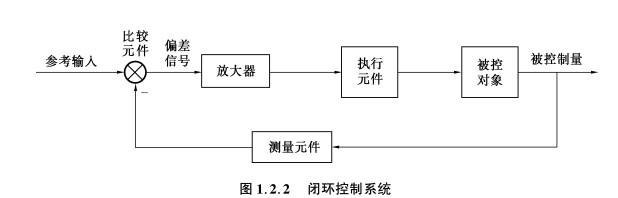
\includegraphics[width=8cm]{闭环控制系统.png}
        \caption{闭环控制系统结构框图}
    \end{figure}
    \vspace{-10pt}

    经典控制理论
    \subsection{控制系统的元件和信号}
    \vspace{-10pt}
    \begin{table}[H]
        \centering
        \caption{}
        \begin{tabular}{|c|c|}
        \hline    
            测量元件 & 检测被控制的物理量 \\
            \hline
            给定元件 & 给出与期望的被控量相对应的系统输入量 \\
            \hline
            比较元件 & 求出测量元件测量的被控量实际值与给定元件给出的输入量的偏差 \\
            \hline
            放大元件 & 将比较元件给出的偏差信号进行放大，推动执行元件控制被控对象 \\
            \hline
            执行元件 & 直接推动被控对象使其被控量发生变化 \\ 
            \hline
            校正元件 & 用串联或反馈的方式连接在系统中，以改善系统的性能 \\
        \hline
        \end{tabular}
    
        \caption{系统的信号}
        \begin{tabular}{|c|c|}
        \hline    
            输入信号 & $r(t)$ \\
            \hline
            输出信号 & $y(t)$ \\
            \hline
            反馈信号 & $b(t)$ \\
            \hline
            偏差信号 & $\varepsilon(t)=r(t)-f(t)$ \\
            \hline
            误差信号 & $e(t)=y_r(t)-y(t)$ \\ 
            \hline
            干扰信号 & $f(t)$ \\
        \hline
        \end{tabular}
    \end{table}

    \subsection{控制系统的基本要求}
        (1)稳定性；(2)快速性；(3)平稳性；(4)准确性。  
\newpage  
\section{线性连续系统的数学模型}
    \subsection{微分方程与传递函数}
        \subsubsection{微分方程模型}
        根据实际物理规律列出微分方程，通式为：
 
        \[
        a_ny^{(n)}+a_{n-1}y^{(n-1)}+\cdots+a_1y'+a_0y=b_mr^{(n)}+b_{m-1}r^{(m-1)}+\cdots+b_1r'+b_0r
        \]


        \begin{figure}[H]
            \centering
            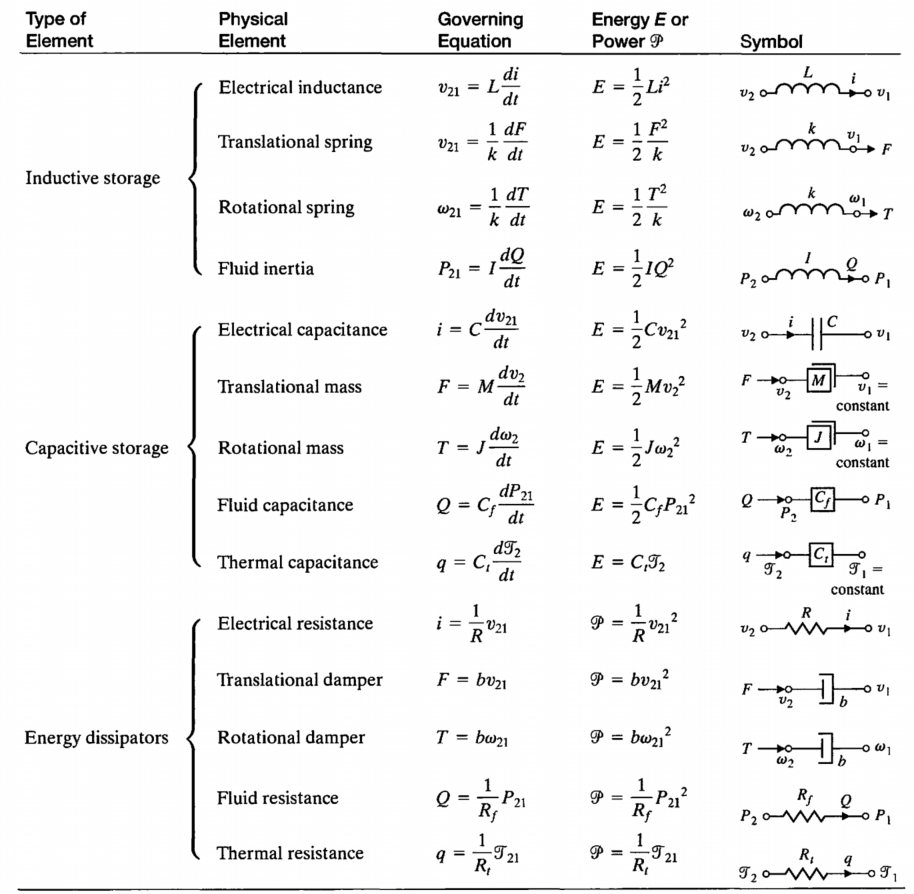
\includegraphics[width=8cm]{三大系统.png}
            \caption{三种常见系统的模型}
        \end{figure}
        \subsubsection{拉普拉斯变换（Laplace Transform）}
            正变换：$F(s)=\mathscr{L}[f(t)]=\int_{0^-}^{\infty}f(t)\e^{-st}\d t$

            逆变换：$f(t)=\mathscr{L}^{-1}[F(s)]=\dfrac{1}{2\pi\j}\int_{\sigma-\j\infty}^{\sigma+\j\infty}F(s)\e^{st}\d s$

            {\setlength{\parindent}{0pt}\textbf{拉普拉斯变换的性质}}
            \begin{itemize}
                \item 线性：$af(t)+bg(t)\xleftrightarrow{\mathscr{L}}aF(s)+bG(s)$
                \item 时移性质：$f(t-t_0)\xleftrightarrow{\mathscr{L}}\e^{-st_0}F(s)$
                \item 尺度变换：$f(at)\xleftrightarrow{\mathscr{L}}\dfrac{1}{a}F(\dfrac{s}{a})$
                \item 频移性质：$\e^{-at}f(t)\xleftrightarrow{\mathscr{L}}F(s+a)$
                \item 微分性质：$\dfrac{\d^n}{\d t^n}f(t)\xleftrightarrow{\mathscr{L}}s^nF(s)-s^{n-1}f(0^-)-s^{n-2}f'(0^-)-\cdots-f^{(n-1)}(0^-)$
                \item 积分性质：$\int_0^tf(\tau)\d\tau\xleftrightarrow{\mathscr{L}}\dfrac{F(s)}{s}$
                \item 卷积定理：$f(t)*g(t)\xleftrightarrow{\mathscr{L}}F(s)G(s)$
                \item 初值定理：$\lim\limits_{t\rightarrow0^+}f(t)=\lim\limits_{s\rightarrow\infty}sF(s)$
                \item 终值定理：$F(s)$在虚轴和右半平面不存在极点且在原点处至多有一阶极点，$\lim\limits_{t\rightarrow\infty}f(t)=\lim\limits_{s\rightarrow0}sF(s)$
            \end{itemize}
        \subsubsection{复数域模型}
        在零初始值的条件下，对微分方程进行拉氏变换得到复数域模型：

        \[
        (a_ns^{n}+a_{n-1}s^{n-1}+\cdots+a_1s+a_0)Y(s)=(b_ms^{n}+b_{m-1}s^{m-1}+\cdots+b_1s+b_0)R(s)
        \]
        
        则传递函数$G(s)=\dfrac{Y(s)}{R(s)}=\dfrac{b_ms^{n}+b_{m-1}s^{m-1}+\cdots+b_1s+b_0}{a_ns^{n}+a_{n-1}s^{n-1}+\cdots+a_1s+a_0}$

        两种常用形式：
        \begin{itemize}
            \item 尾1标准型（时间常数形式）：
            $G(s)=\dfrac{b_0}{a_0}\dfrac{d_ms^{n}+d_{m-1}s^{m-1}+\cdots+d_1s+1}{c_ns^{n}+c_{n-1}s^{n-1}+\cdots+c_1s+1}=K\dfrac{\prod\limits_{i=1}^m(T_is+1)}{\prod\limits_{j=1}^n(t_js+1)}$
            \item 首1标准型（零极点形式）：
            $G(s)=\dfrac{b_n}{a_n}\dfrac{s^{n}+h_{m-1}s^{m-1}+\cdots+h_1s+h_0}{s^{n}+l_{n-1}s^{n-1}+\cdots+l_1s+l_0}=K_g\dfrac{\prod\limits_{i=1}^m(s-z_i)}{\prod\limits_{j=1}^n(s-s_j)}$
        \end{itemize}

        传递函数一般为有理真分式，分母次数大于等于分子次数，传递函数只取决于系统的结构和参数，与输入、输出的位置有关，但与输入信号无关，与单位脉冲响应互为拉氏变换对。
        \subsubsection{典型环节}
            \begin{enumerate}
                \item 比例环节：$y(t)=Kr(t),G(s)=K$
                \item 惯性环节：$Ty'(t)+y(t)=r(t),G(s)=\dfrac{1}{Ts+1}$
                \item 积分环节：$Ty'(t)=r(t),G(s)=\dfrac{1}{Ts}$
                \item 振荡环节：$T^2y''(t)+2T\zeta y'(t)+y(t)=r(t)(0<\zeta<1),G(s)=\dfrac{1}{Ts^2+2\zeta Ts+1}=\dfrac{\omega_n^2}{s^2+2\zeta\omega_ns+\omega_n^2}$
                \item 微分环节：$y(t)=Tr'(t),G(s)=Ts$
                \item 一阶复合微分环节：$G(s)=\dfrac{T_1s}{T_2s+1}$
                \item 延迟环节：$y(t)=r(t-\tau),G(s)={\rm e}^{-\tau s}$
            \end{enumerate}      
    \subsection{系统框图}
        \subsubsection{框图的结构变换}
            开环传递函数$G(s)H(s)$，闭环传递函数$\varPhi(s)=\dfrac{Y(s)}{R(s)}=\dfrac{G(s)}{1+G(s)H(s)}$

            方框图：每个环节用方框表示，框中表明环节的传递函数，根据信号传递关系将各方框连接起来。
\newpage
            \begin{figure}[H]
                \centering
                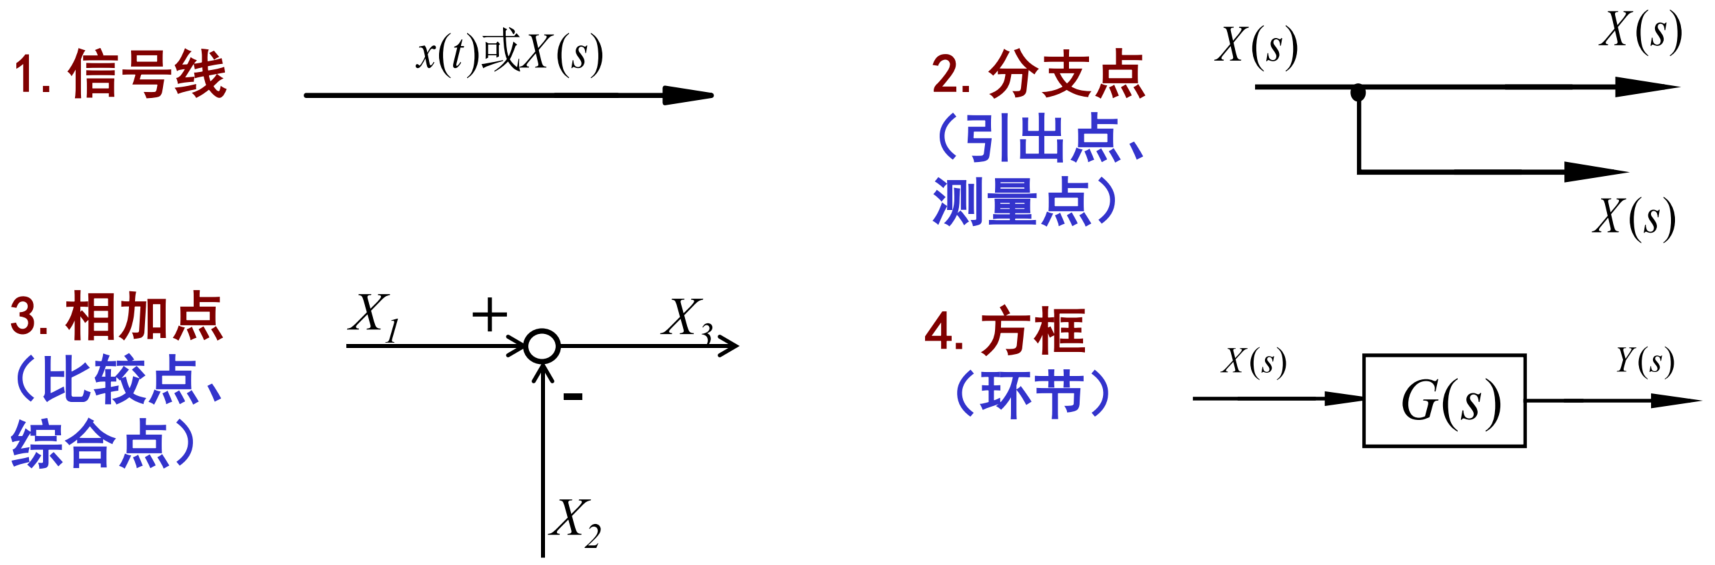
\includegraphics[width=8cm]{框图基本元素.png}
                \caption{方框图的基本单元}
            \end{figure}

            节点：用以表示信号或变量的点。节点所表示的变量等于流入该节点的信号之和，从节点流出的每一条分支的信号都等于该节点所表示的变量。

            支路：连接两个节点，并在中间用箭头标出信号流向的定向线段。支路的增益称为传输。

            通路：沿箭头所指方向从一个节点穿过各相连支路到另一个节点。

            前向通路：信号从输入节点向输出节点传递且每个节点只通过一次的通路。

            回路：起点和终点是同一节点且信号通过每个节点不多于一次的闭合通路。
            \begin{figure}[H]
                \centering
                \begin{subfigure}[b]{0.48\textwidth}
                    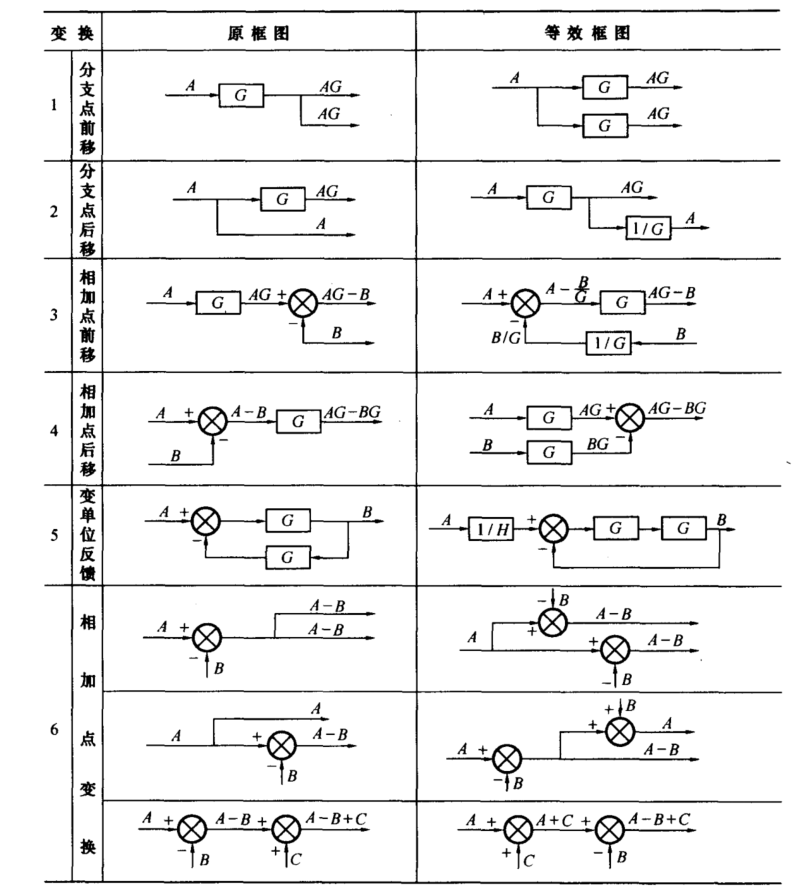
\includegraphics[width=\textwidth]{框图基本变换.png}
                    \caption{方框图的结构变换}
                \end{subfigure}
                \hfill
                \begin{subfigure}[b]{0.48\textwidth}
                    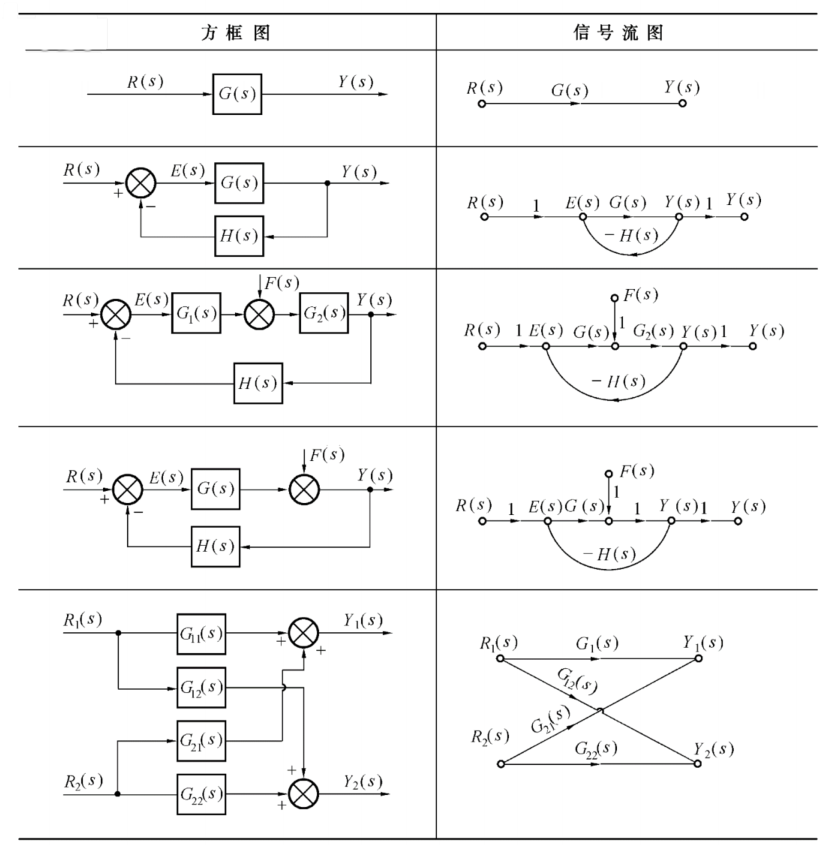
\includegraphics[width=\textwidth]{框图和信号流图.png}
                    \caption{方框图和信号流图的转换}
                \end{subfigure}
            \end{figure}

        \subsubsection{梅森（Mason）公式}
            $P=\dfrac1\Delta\sum P_k\Delta_k$

            $\Delta$系统框图的特征式，$\Delta=1-\sum\limits_aL_a+\sum\limits_{bc}L_bL_c-\sum\limits_{def}L_dL_eL_f+\cdots$

            $\sum\limits_aL_a$所有回路增益之和；
            
            $\sum\limits_{bc}L_bL_c$每两个互不接触的回路增益乘积之和；$\sum\limits_{def}L_dL_eL_f$每三个互不接触回路增益乘积之和；

            $P_k$第$k$条前向回路的通路增益；

            $\Delta_k$在$\Delta$中去除与第$k$条前向通路相接触的（有公共节点）回路后的特征式，称为余因式。
\newpage
\section{线性连续系统的时域分析}
    \begin{table}[H]
        \centering
        \caption{典型输入信号}
        \resizebox{0.5\textwidth}{!}{
        \begin{tabular}{|c|c|c|}
        \hline    
            信号名称 & 像原函数 & 像函数\\
            \hline
            单位冲激信号 & $\delta(t)=\begin{cases}\infty&t=0\\0&t\neq0\end{cases}\qquad \int_{-\infty}^{+\infty}\delta(t){\rm{d}}t=1$ & $1$ \\
            \hline
            单位阶跃信号 & $u(t)=1(t)=\begin{cases}1&t>0\\0&t<0\end{cases}$ & $\dfrac{1}{s}$ \\
            \hline
            单位斜坡信号 & $r(t)=\begin{cases}t&t>0\\0&t<0\end{cases}$ & $\dfrac{1}{s^2}$ \\
            \hline
            单位加速度信号 & $r(t)=\begin{cases}\dfrac12t^2&t>0\\0&t<0\end{cases}$ & $\dfrac{1}{s^3}$ \\
        \hline
        \end{tabular}
        }
    \end{table}

    线性定常系统(LTI)的特性：系统对输入信号导数的响应等于系统对该输入信号响应的导数；系统对输入信号积分的响应等于系统对该输入信号响应的积分。
    \subsection{动态性能指标}
        延迟时间$t_d$：系统响应从$0$上升到稳态值的$50\%$所需的时间。

        上升时间$t_r$：对于振荡系统，系统响应从$0$上升到稳态所需的时间；对于无振荡系统，系统响应从稳态值的$10\%$上升到$90\%$所需的时间。

        峰值时间$t_p$：系统响应第一次达到最大峰值的时间。

        调节时间$t_s$：系统响应与稳态值之差达到并维持误差$\Delta$所需的最小时间。

        （最大）超调量$\sigma\%$：系统响应超出稳态值的最大偏移量，$\sigma\%:=\dfrac{y(t_p)-y(\infty)}{y(\infty)}\times100\%$

        振荡次数$N$：调节时间$t_s$内，响应偏离稳态值的次数。
    \subsection{一阶系统}
        \subsubsection{单位阶跃相应}
            系统闭环传递函数$G(s)=\dfrac{1}{Ts+1}$

            输入$r(t)=u(t),R(s)=\dfrac1s$
            
            输出$Y(s)=G(s)R(s)=\dfrac{1}{(Ts+1)s},y(t)=1-{\rm e}^{-\frac tT}$
            
            误差$e(t)=1-y(t)={\rm e}^{-\frac tT}$

            \begin{figure}[H]
                \centering
                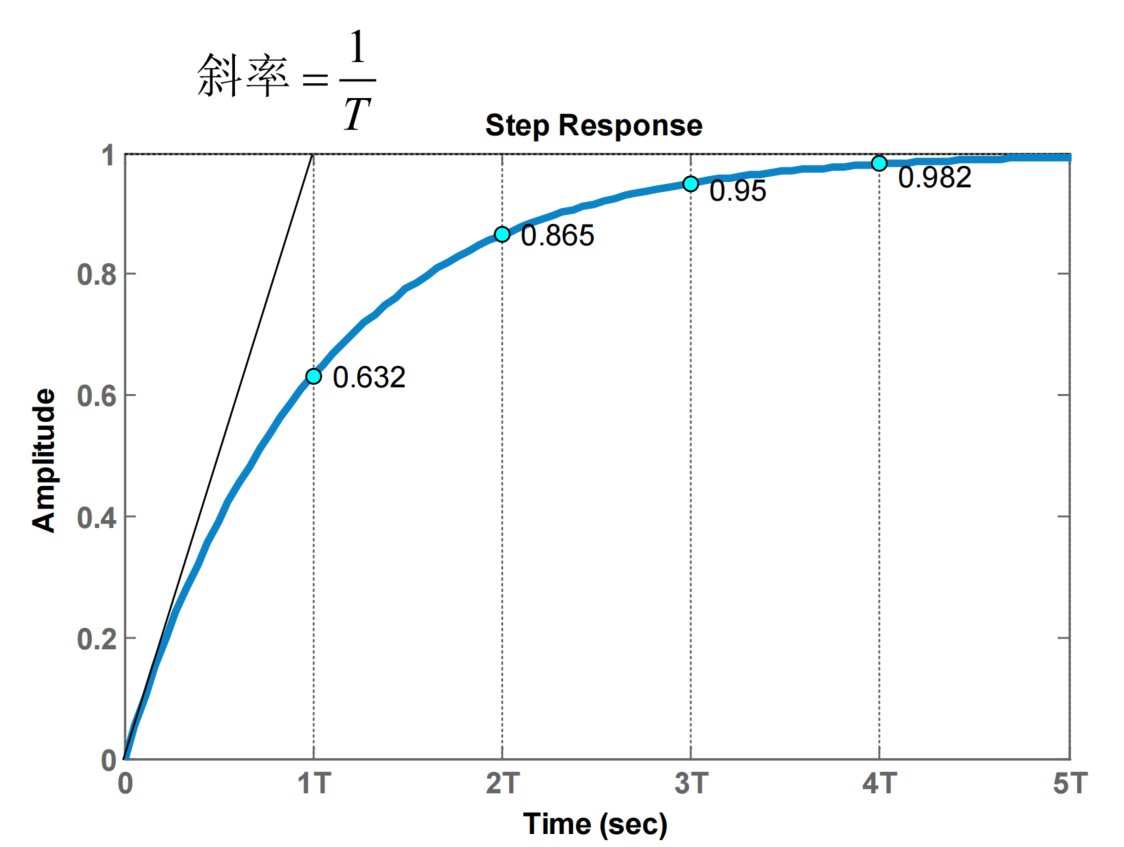
\includegraphics[width=5cm]{一阶阶跃.png}
                \caption{单位阶跃响应}
            \end{figure}
        {\setlength{\parindent}{0pt}\textbf{单位阶跃响应动态指标}}

            $t_d=-T\ln 0.5=0.69T$
            
            $t_r=t_{0.9}-t_{0.1}=-T\ln\frac{0.1}{0.9}=2.2T$
            
            $t_s=3T(\Delta=5\%)$
        \subsubsection{一阶系统单位响应的特点}
            单位阶跃响应：$y(t)=1-{\rm e}^{-\frac tT}$，输出$y(t)$是初值为$0$、终值为$1$的单调连续上升过程，稳态误差为$0$.

            单位脉冲响应：$y(t)=\dfrac1T{\rm e}^{-\frac tT}$，输出$y(t)$是初值为$1/T$、终值为$0$的单调连续下降过程，稳态误差为$0$。
            
            单位斜坡响应：$y(t)=t-T(1-{\rm e}^{-\frac tT})$，输出$y(t)$是初值为$0$的单调连续上升过程，终值趋于$r(t)-T$，稳态误差为$T$。
            \begin{figure}[H]
                \centering
                \begin{subfigure}[b]{0.48\textwidth}
                    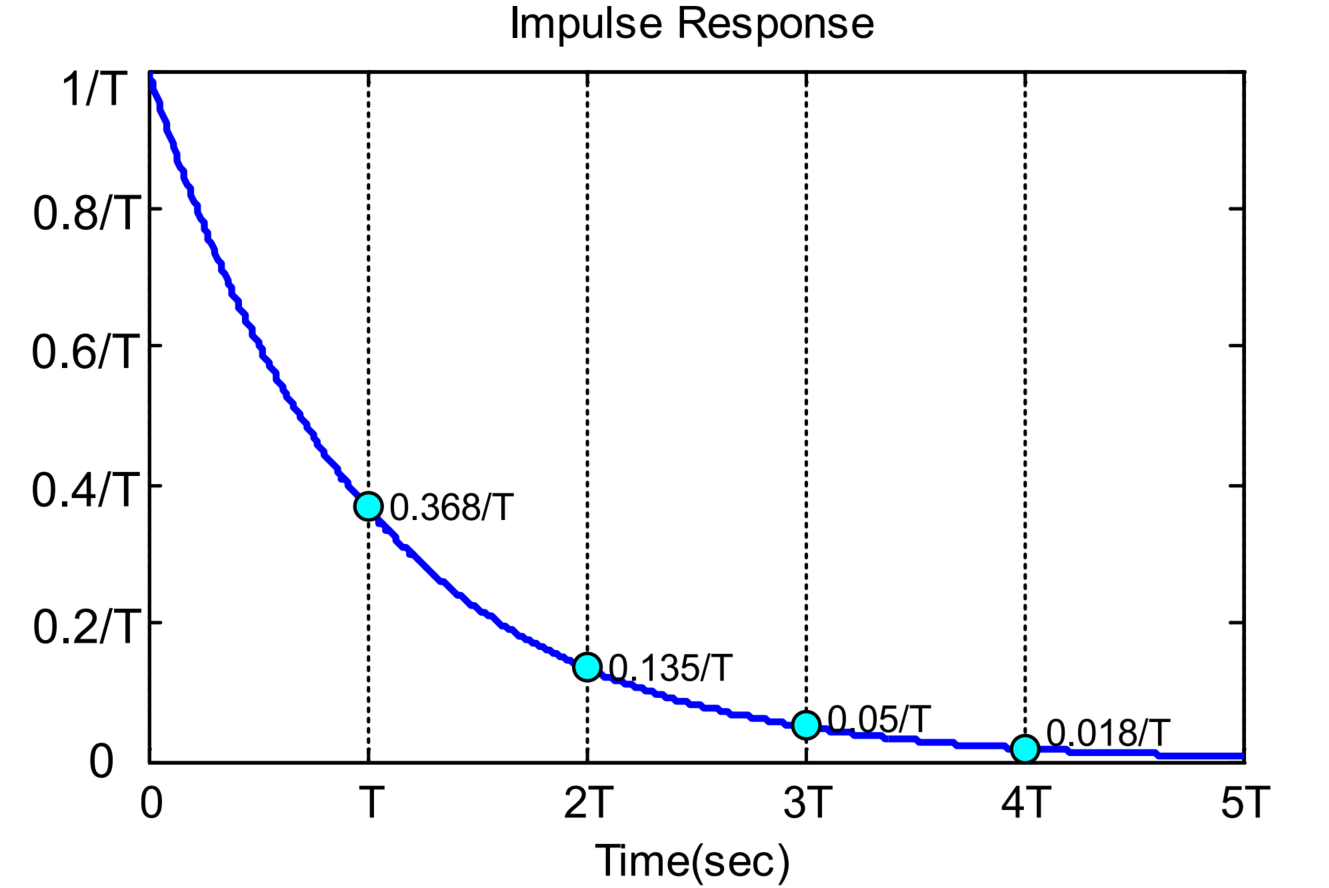
\includegraphics[width=\textwidth]{一阶脉冲.png}
                    \caption{单位脉冲响应}
                \end{subfigure}
                \hfill
                \begin{subfigure}[b]{0.48\textwidth}
                    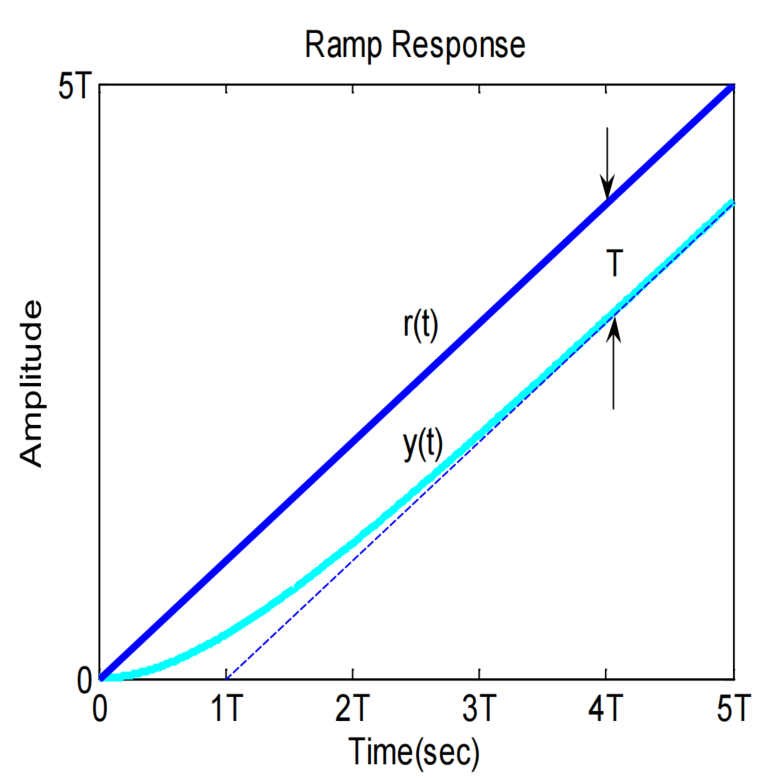
\includegraphics[width=\textwidth]{一阶斜坡.png}
                    \caption{单位斜坡响应}
                \end{subfigure}
            \end{figure}
    \subsection{二阶系统}
        闭环传递函数：$G(s)=\dfrac{\omega_n^2}{s^2+2\zeta\omega_ns+\omega_n^2}$，其中$\omega_n$为无阻尼振荡频率，$\zeta$为阻尼比

        特征方程：$D(s)=s^2+2\zeta\omega_ns+\omega_n^2$，极点$s_{1,2}=-\zeta\omega_n\pm\omega_n\sqrt{\zeta^2-1}$
        \subsubsection{二阶系统的单位阶跃响应}
            \begin{figure}[H]
                \centering
                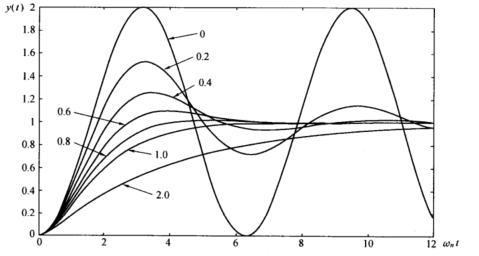
\includegraphics[width=7cm]{二阶阶跃.png}
                \caption{二阶系统的单位阶跃响应}
            \end{figure}
            {\setlength{\parindent}{0pt}\textbf{3.3.1.1\quad 过阻尼（$\zeta>1$）}}

                $y(t)=1-\dfrac{\omega_n}{2\sqrt{\zeta^2-1}}\big(T_1{\rm e}^{-\frac t T_1}-T_2{\rm e}^{-\frac t T_2}\big)$
                
                其中时间常数$T_1=-\dfrac{1}{s_1}=\dfrac{1}{\omega_n(\zeta-\sqrt{\zeta^2-1})},T_2=-\dfrac{1}{s_2}=\dfrac{1}{\omega_n(\zeta+\sqrt{\zeta^2-1})}$

                以负指数上升至稳态值$1$，无振荡，无稳态误差。
            
            {\setlength{\parindent}{0pt}\textbf{3.3.1.2\quad 临界阻尼（$\zeta=1$）}}

                $s_{1,2}=-\omega_n,y(t)=1-{\rm e}^{-\omega_nt}(1+\omega_nt)$

            {\setlength{\parindent}{0pt}\textbf{3.3.1.3\quad 欠阻尼（0<$\zeta<1$）}}

                $s_{1,2}=-\zeta\omega_n\pm{\rm j}\omega_n\sqrt{1-\zeta^2}=-\sigma\pm{\rm j}\omega_d$

                $y(t)=1-\dfrac{{\rm e}^{-\zeta\omega_nt}}{\sqrt{1-\zeta^2}}\sin(\omega_dt+\arccos\zeta)$

                以指数为包络线衰减的正弦振荡，衰减速度取决于阻尼系数$\sigma=\zeta\omega_n$，稳态分量为$1$，无稳态误差。

                \textbf{欠阻尼过程的动态性能：}

                峰值时间：令$\dfrac{{\rm d}y(t)}{{\rm d}t}\big|_{t=t_p}=0$，得$t_p=\dfrac{\pi}{\omega_d}=\dfrac{\pi}{\omega_n\sqrt{1-\zeta^2}}$

                超调量：$\sigma\%=(y(t_p)-1)\times100\%={\rm e}^{-\dfrac{\zeta\pi}{\sqrt{1-\zeta^2}}}\times100\%$

                上升时间：$t_r=\dfrac{\pi-\arccos\zeta}{\omega_n\sqrt{1-\zeta^2}}$

                调节时间：取$\dfrac{{\rm e}^{-\zeta\omega_nt_s}}{\sqrt{1-\zeta^2}}\approx\Delta$，得$t_s=\dfrac{1}{\zeta\omega_n}(\ln\dfrac{1}{\Delta\sqrt{1-\zeta^2}})$
                
                忽略$\dfrac12\ln(1-\zeta^2)$项，近似认为$t_s(2\%)\approx\dfrac{4}{\zeta\omega_n},t_s(5\%)\approx\dfrac{3}{\zeta\omega_n}$

                延迟时间：由隐函数决定，$\omega_nt_d=\dfrac{1}{\zeta}\ln\dfrac{2\sin(\omega_dt_d+\arccos\zeta)}{\sqrt{1-\zeta^2}}$

                振荡次数：阻尼振荡周期$\tau_d=\dfrac{2\pi}{\omega_n\sqrt{1-\zeta^2}}$，
                故$N=\dfrac{t_s}{\tau_d}=\begin{cases}\dfrac{2\sqrt{1-\zeta^2}}{\pi\zeta}&\Delta=2\%\\\dfrac{1.5\sqrt{1-\zeta^2}}{\pi\zeta}&\Delta=5\%\end{cases}$
            
            {\setlength{\parindent}{0pt}\textbf{3.3.1.4\quad 零阻尼（$\zeta=0$）}}
            
                正弦等幅震荡无衰减。

                $s_{1,2}=\pm{\rm j}\omega_n,y(t)=1-\cos\omega_nt$，动态指标$\sigma\%=100\%,t_s=\infty$

            {\setlength{\parindent}{0pt}\textbf{3.3.1.1\quad 负阻尼（$\zeta<0$）}}
                
                当$-1<\zeta<0$时，

                $s_{1,2}=-\zeta\omega_n\pm{\rm j}\omega_n\sqrt{1-\zeta^2}=-\sigma_n\pm{\rm j}\omega_d$

                $y(t)=1-\dfrac{{\rm e}^{-\zeta\omega_nt}}{\sqrt{1-\zeta^2}}\sin(\omega_dt+\arccos\zeta)$

                以指数为包络线发散的正弦振荡，发散速度取决于$-\zeta\omega_n$。

                当$\zeta<-1$时，

                $s_{1,2}=\omega_n(-\zeta\pm\sqrt{\zeta^2-1})$

                $y(t)=1+\dfrac{\omega_n}{2\sqrt{\zeta^2-1}}(\dfrac{1}{s_1}{\rm e}^{s_1t}+\dfrac{1}{s_2}{\rm e}^{s_2t})$

                指数发散，发散速度取决于两个极点$s_1,s_2$的大小。
        \subsubsection{具有零点的二阶系统的单位阶跃响应}
            闭环传递函数$G(s)=\dfrac{\omega_n^2(\tau s+1)}{s^2+2\zeta\omega_ns+\omega_n^2}$
    
            $Y_Z(s)=Y(s)+\dfrac szY(s),y_z(t)=y(t)+\dfrac 1z\dot{y}(t)$，其中系统零点$-z=-\dfrac 1\tau$
        
            $y(t)=1-\dfrac{{\rm e}^{-\zeta\omega_nt}}{\sqrt{1-\zeta^2}}\dfrac lz\sin(\omega_dt+\arccos\zeta+\psi)$
            
            其中$\psi=\arccos\dfrac{z-\zeta\omega_n}{l},l=\sqrt{(z-\zeta\omega_n)^2+\omega_d^2}=\sqrt{D(z)},\dfrac lz=\dfrac{\sqrt{\zeta^2-2r\zeta^2+r^2}}{\zeta}$，
            
            $r=\dfrac{\zeta\omega_n}{z}$为复极点实部与零点之比。
            
            {\setlength{\parindent}{0pt}\textbf{添加左半平面的零点对动态性能的影响：}}
            
            上升时间：$t_{rz}=\dfrac{\pi-\arccos\zeta-\phi}{\omega_d}=t_r-\dfrac{\psi}{\omega_d}$

            峰值时间：$t_{pz}=\dfrac{\pi-\psi}{\omega_d}=t_p-\dfrac{\psi}{\omega_d}$

            超调量：$\sigma\%=\dfrac lz{\rm e}^{-\zeta\omega_nt_{pz}}=\dfrac lz{\rm e}^{\frac{\zeta\psi}{\sqrt{1-\zeta^2}}}\times\sigma\%$

            调节时间：$\dfrac{1}{\zeta\omega_n}(\ln\dfrac{1}{\Delta(1-\zeta^2)}-\ln\dfrac lz)=t_s-\dfrac{1}{\zeta\omega_n}\ln\dfrac lz$

            总而言之，峰值时间提前；超调量增大，振荡加剧；$r=\dfrac{\zeta\omega_n}{z}$越大影响越大。
        \subsubsection{二阶系统的单位脉冲响应}
            $Y(s)=\dfrac{\omega_n^2}{s^2+2\zeta\omega_ns+\omega_n^2}$
            \begin{figure}[H]
                \centering
                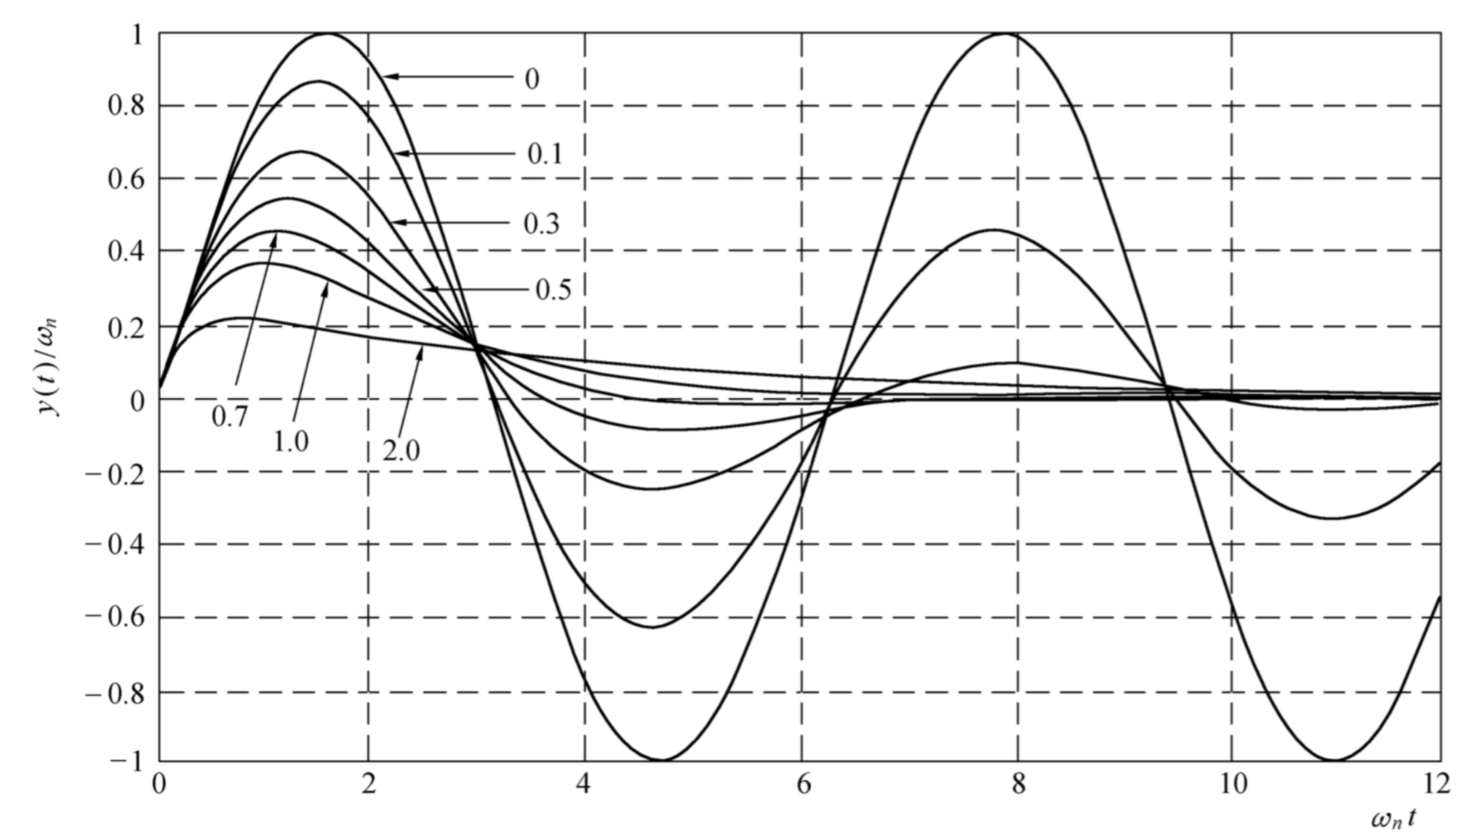
\includegraphics[width=8cm]{二阶脉冲.png}
                \caption{二阶系统的单位脉冲响应}
            \end{figure}
            \begin{itemize}
            \item 无阻尼：$y(t)=\omega_n\sin(\omega_nt)$
            \item 欠阻尼：$y(t)=\dfrac{\omega_n}{\sqrt{1-\zeta^2}}\e^{-\zeta\omega_nt}\sin(\omega_dt)$
            \item 临界阻尼：$y(t)=\omega_n^2t\e^{-\omega_nt}$
            \item 过阻尼：$y(t)=\dfrac{\omega_n}{2\sqrt{\zeta^2-1}}\bigg[\e^{-(\zeta-\sqrt{\zeta^2-1})\omega_nt}-\e^{-(\zeta+\sqrt{\zeta^2+1})\omega_nt}\bigg]$
            \end{itemize}
            单位脉冲响应是单位阶跃响应对时间的导数，第一次过零点时间是单位脉冲响应的峰值时间。单位脉冲响应是系统传递函数的拉氏变换，可以反映系统的全部特性。
        \subsubsection{二阶系统的单位斜坡响应}
            $Y(s)=\dfrac{1}{s^2}G(s)=\dfrac{1}{s^2}-\dfrac{2\zeta}{\omega_ns}+\dfrac{2\zeta(s+\zeta\omega_n)+\omega_n(2\zeta^2-1)}{\omega_n(s^2+2\zeta\omega_ns+\omega_n^2)}$
            \begin{itemize}
            \item 欠阻尼：$y(t)=t-\dfrac{2\zeta}{\omega_n}+\dfrac{1}{\omega_n\sqrt{1-\zeta^2}}\e^{-\zeta\omega_nt}\sin(\omega_dt+\arctan\dfrac{2\zeta\sqrt{1-\zeta^2}}{2\zeta^2-1})$
            \item 临界阻尼：$y(t)=t-\dfrac{2}{\omega_n}+\dfrac{2}{\omega_n}\e^{-\omega_nt}(1+\dfrac{\omega_nt}{2})$
            \item 过阻尼：$y(t)=t-\dfrac{2\zeta}{\omega_n}-\dfrac{2\zeta^2-1-2\zeta\sqrt{\zeta^2-1}}{2\omega_n\sqrt{\zeta^2-1}}\e^{-(\zeta+\sqrt{\zeta^2-1})\omega_nt}
            +\dfrac{2\zeta^2-1+2\zeta\sqrt{\zeta^2-1}}{2\omega_n\sqrt{\zeta^2-1}}\e^{-(\zeta+\sqrt{\zeta^2+1})\omega_nt}$
            \end{itemize}
    \subsection{高阶系统}
        \subsubsection{典型三阶系统}
            以惯性环节和二阶环节串联的三阶典型系统分析：
        
            $G(s)=\dfrac{\omega_n^2}{(Ts+1)(s^2+2\zeta\omega_ns+\omega_n^2)}$

            $y(t)=1-\dfrac{{\rm e}^{-\beta\zeta\omega_nt}}{\zeta^2\beta(\beta-2)+1}-\dfrac{\beta\zeta}{\sqrt{\zeta^2\beta(\beta-2)+1}}
            \dfrac{{\rm e}^{-\zeta\omega_nt}}{\sqrt{1-\zeta^2}}\sin(\omega_dt+\gamma)$
            
            其中$\gamma=\arctan\dfrac{\zeta(\beta-2)\sqrt{1-\zeta^2}}{\zeta^2(\beta-2)+1},\beta=\dfrac{p}{\zeta\omega_n}=\dfrac{1}{T\zeta\omega_n}$

            $\beta>>1$，共轭复数极点为主导极点，响应主要呈现二阶特性；$\beta<<1$，实极点为主导极点，响应主要呈现一阶特性

            当$\beta\ge5$或$\beta\le\dfrac15$时，可按照主导共轭复数极点或主导实极点估算暂态特性。

            实极点使系统振荡性减弱，超调量减小，响应速度变慢，增加了系统的惯性。
        \subsubsection{一般的高阶系统}
            对于一般的高阶系统，传递函数如下：

            \[
            Y(s)=\dfrac{k\prod\limits_{i=1}^m(s-z_i)}{\prod\limits_{j=1}^q(s-s_j)\prod\limits_{k=1}^{r}(s^2+2\zeta_k\omega_{nk}s+\omega_{nk}^2)}\cdot\dfrac1s
            =\dfrac1s+\sum\limits_{j=1}^{q}\dfrac{A_j}{s-s_j}+\sum\limits_{k=1}^{r}\dfrac{B_k(s+\zeta_k\omega_{nk})+C_k\omega_{nk}\sqrt{1-\zeta_k^2}}{s^2+2\zeta_k\omega_{nk}s+\omega_{nk}^2}
            \]

            经过拉式反变换得$y(t)=1+\sum\limits_{j=1}^{q}\dfrac{A_j}{s-s_j}+\sum\limits_{k=1}^{r}D_k{\rm e}^{-\zeta_k\omega_{nk}t}\sin(\omega_{nk}t+\theta_k)$
            
            $A_j=k\dfrac{(s-z_1)(s-z_2)\cdots(s-z_m)}{s(s-s_1)(s-s_2)\cdots(s-s_n)}(s-s_j)\big|_{s=s_j},
            D_k=2\bigg|k\dfrac{(s-z_1)(s-z_2)\cdots(s-z_m)}{s(s-s_1)(s-s_2)\cdots(s-s_n)}(s-s_k)\big|_{s=s_k}\bigg|$
            
            {\setlength{\parindent}{0pt}\textbf{高阶系统的定性分析}}

                (1)如果高阶系统的闭环极点全部具有负实部，即极点全部在复平面的左半平面，则系统单位阶跃响应的暂态分量最终全部衰减为$0$，系统最终有稳态值
            
                (2)在暂态分量中，每一项衰减的快慢取决于相应实数闭环极点的绝对值$|s_i|$或复数闭环极点的实部绝对值$|\zeta_k\omega_{nk}|$，系统闭环极点在复平面左半平面离虚轴越远，相对应的指数项衰减越快
            
                (3)如果某一闭环极点靠近一零点，且与其他极点相距较远，则相应项的系数较小，在暂态分量中影响较小；一对非常接近的闭环零极点称作一对偶极子，偶极子对暂态过程几乎没有影响 
                
            \begin{figure}[H]
                \centering
                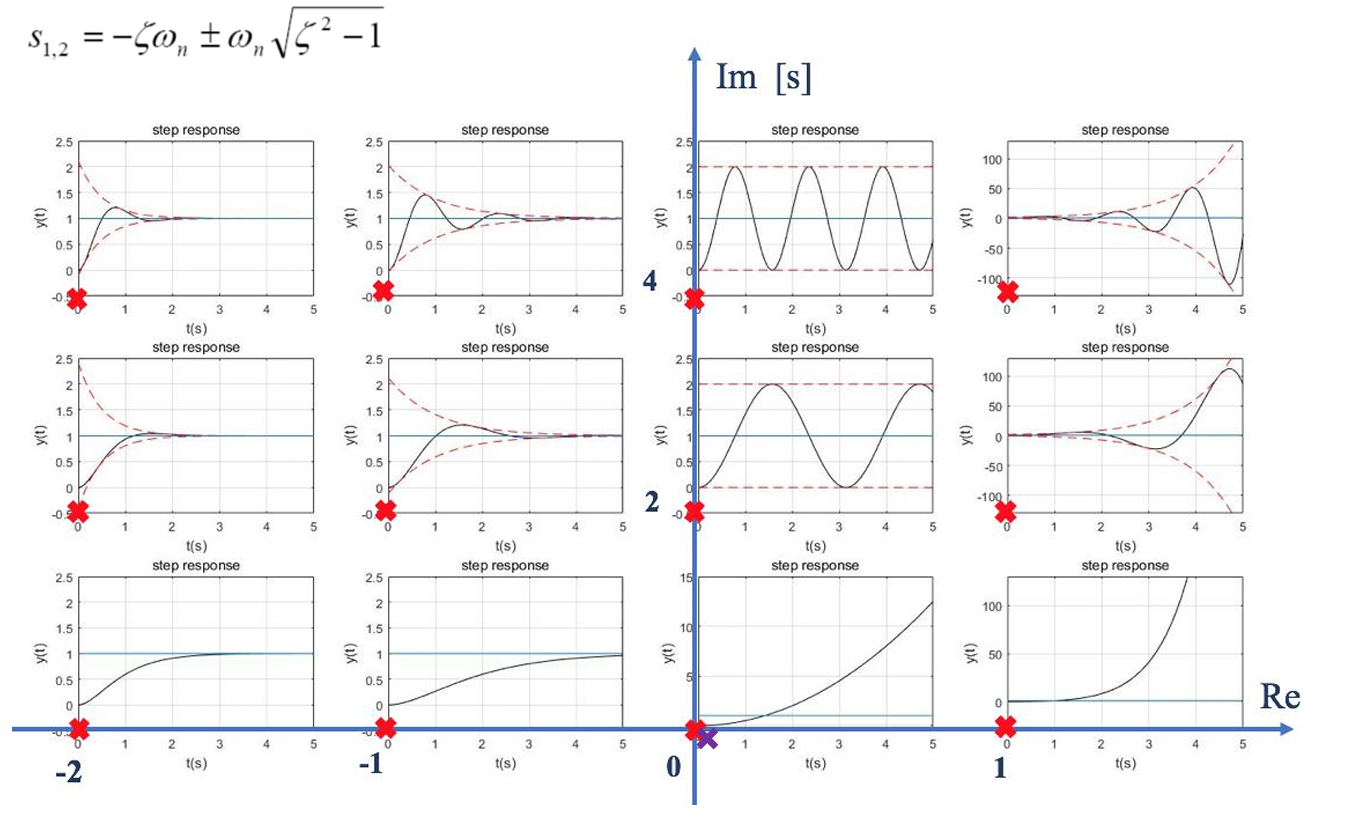
\includegraphics[width=8cm]{极点与阶跃响应.png}
                \caption{系统阶跃响应和极点的关系}

                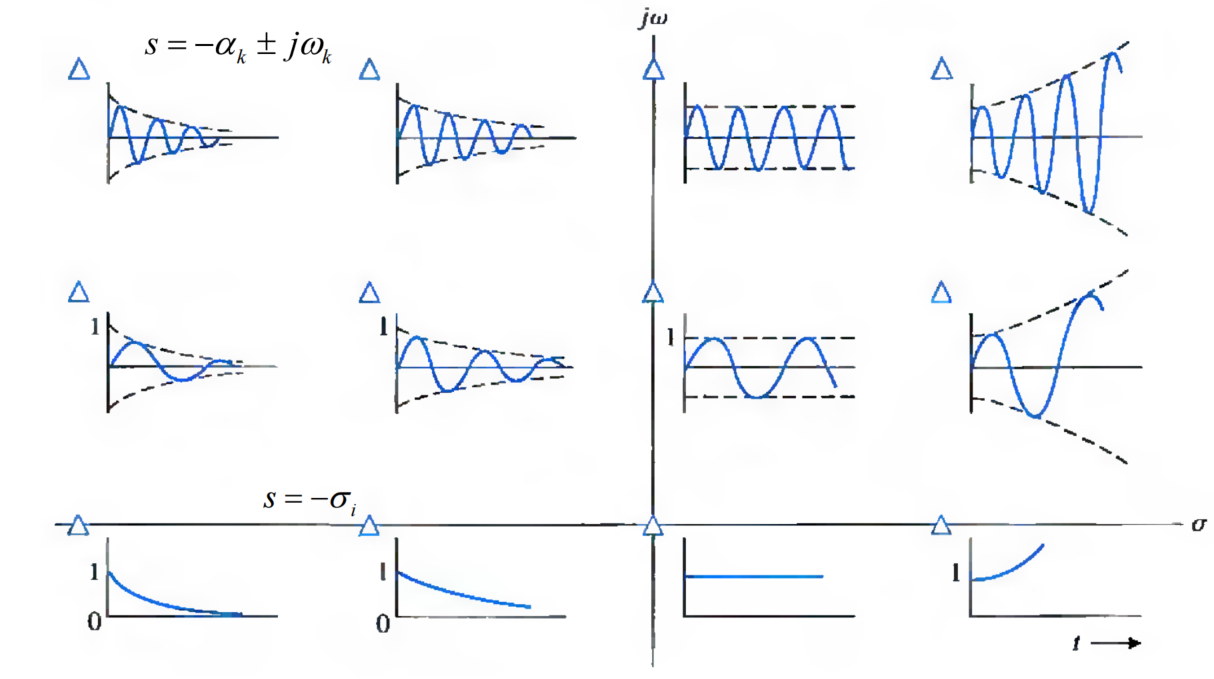
\includegraphics[width=8cm]{极点与脉冲响应.png}
                \caption{系统脉冲响应和极点的关系}  
            \end{figure}
    \subsection{时域稳定性分析}
        稳定性定义：在扰动作用下系统偏离原来的平衡状态，扰动消除后系统能够恢复到原来的平衡状态。

        判定线性定常系统稳定性的数学依据是：$\lim\limits_{t\rightarrow\infty}k(t)=0$。

        线性定常系统稳定的充要条件是：闭环系统特征方程的根全部具有负实部，或者说闭环传递函数的极点全部在复平面的左半平面。
        \subsubsection{劳斯（Routh）判据}
            (1)特征方程不缺项；(2)各项系数全是正实数；(3)劳斯表第一列各元均大于零。
            \begin{table}[H]
                \centering
                \caption{劳斯表}
                \begin{tabular}{c c c c c c}
                    $s^n$ & $a_n$ & $a_{n-2}$ & $a_{n-4}$ & $a_{n-6}$ & $\cdots$\\
                    $s^{n-1}$ & $a_{n-1}$ & $a_{n-3}$ & $a_{n-5}$ & $a_{n-7}$ & $\cdots$\\
                    $s^{n-2}$ & $b_1$ & $b_2$ & $b_3$ & $\cdots$ & $\cdots$\\
                    $\vdots$ & $c_1$ & $c_2$ & $\cdots$ & $\cdots$ & $\cdots$\\
                    $s^2$ & $\vdots$ & $\vdots$ & $\vdots$ & $\ddots$ & \\
                    $s^1$ & $\vdots$ & $\vdots$ & $\vdots$ &  & $\ddots$\\
                    $s^0$ & $\vdots$ & $\vdots$ & $\vdots$ & $\cdots$ & $\cdots$\\
                \end{tabular}
            \end{table}
            
            其中，$b_1=\dfrac{a_{n-1}a_{n-2}-a_na_{n-3}}{a_{n-1}},b_2=\dfrac{a_{n-1}a_{n-4}-a_na_{n-5}}{a_{n-1}},b_3=\dfrac{a_{n-1}a_{n-6}-a_na_{n-7}}{a_{n-1}}$

            $c_1=\dfrac{b_1a_{n-3}-a_{n-1}b_2}{b_1},c_2=\dfrac{b_1a_{n-5}-a_{n-1}b_3}{b_1}$，其他项以此类推
            
            劳斯表的特征：(1)劳斯表的某一行的所有元同乘（除）一个正数不改变 Routh 稳定判据的判定结果；(2)劳斯表第一列元自上而下符号改变的次数等于具有正实部根的极点的个数。

            特殊情况：

            \begin{itemize}
                \item 劳斯表某一行的第一项为$0$：

                以小量$\varepsilon$代替$0$，列写劳斯表完成后令$\varepsilon\rightarrow0^+$判断符号。
                \item 劳斯表的某一行各项全为$0$：

                利用全零行上一行的系数构造一个辅助方程$F(s)=0$，对辅助方程求导后的系数作为全零行各元。其中辅助方程的根是系统虚轴上的极点。
            \end{itemize}
        \subsubsection{赫尔维茨（Hurwitz）判据}
            (1)特征方程不缺项；(2)各项系数全是正实数；(3)赫尔维茨行列式的顺序主子式均为正。
            
            \[
            \Delta_H=\begin{vmatrix}
                a_{n-1} & a_{n-3} & a_{n-5} & \cdots & 0 \\
                a_{n} & a_{n-2} & a_{n-4} & \cdots & 0 \\
                0 & a_{n-1} & a_{n-3} & \cdots & 0 \\
                0 & a_{n} & a_{n-2} & \cdots & 0 \\
                \vdots & \vdots & \vdots & \ddots & \vdots \\
                0 & 0 & 0 & \cdots & a_0 \\
            \end{vmatrix}
            \]

            利纳德-奇帕特（Li\'enard-Chipart）判据：在特征方程各项系数为正的条件下，若所有赫尔维茨行列式的奇次顺序主子式为正，则所有偶次顺序主子式必然为正，反之亦然。
    \subsection{稳态误差}
        按输入端定义，$E(s)=R(s)-H(s)Y(s)$，按输出端定义，$E'(s)=\dfrac{R(s)}{H(s)}-Y(s)$。对单位反馈系统，$E(s)=E'(s)$   

        稳态误差：稳定系统在输入/干扰作用后，在$t\rightarrow\infty$时响应的期望值与实际值的误差。
        
        $e_{ss}=\lim\limits_{t\rightarrow\infty}e(t)=\lim\limits_{t\rightarrow\infty}y_r(t)-y(t)$

        对于单位负反馈系统，$H(s)=1,e(t)=\varepsilon(t)$，则$e_{ss}=\lim\limits_{t\rightarrow\infty}\varepsilon(t)$，以下仅讨论单位负反馈系统稳态误差。
        \subsubsection{静态稳态误差}
            开环传递函数$G(s)=\dfrac{K\prod\limits_{i=1}^m(\tau_is+1)}{s^v\prod\limits_{j=1}^q(T_js+1)\prod\limits_{k=1}^r(T_k^2s^2+2\zeta_kT_ks+1)}$

            其中$v$是开环传递函数中串联积分环节的个数。
        
            $\varepsilon(s)=\varPhi_\varepsilon(s)R(s)$
            故$e_{ss}=\lim\limits_{t\rightarrow\infty}e(t)=\lim\limits_{s\rightarrow0}s\varPhi_\varepsilon(s)R(s)=\lim\limits_{s\rightarrow0}s\dfrac{1}{1+G(s)}R(s)$
        
            $=\lim\limits_{s\rightarrow0}\dfrac{s^v\prod\limits_{j=1}^q(T_js+1)\prod\limits_{k=1}^r(T_k^2s^2+2\zeta_kT_ks+1)}
            {s^v\prod\limits_{j=1}^q(T_js+1)\prod\limits_{k=1}^r(T_k^2s^2+2\zeta_kT_ks+1)+K\prod\limits_{i=1}^m(\tau_is+1)}R(s)$

            由此看出，只要$R(s)$分母阶次小于等于$v$，系统稳态误差就等于$0$，把偏差闭环传递函数分母$s$因子的阶数$v$称作系统的无差度，称系统是$v$阶无静差。
            $v=0,1,2$的系统分别称作0型、I型、II型系统。

            单位阶跃响应，$e_{ss}=\lim\limits_{s\rightarrow0}sE(s)=\lim\limits_{s\rightarrow0}\dfrac{1}{1+G(s)}=\dfrac{1}{1+K_p}$，
            
            其中静态位置误差系数$K_p:=\lim\limits_{s\rightarrow0}G(s)=\begin{cases}K&v=0\\\infty&v\geqslant1\end{cases}$

            单位斜坡响应，$e_{ss}=\lim\limits_{s\rightarrow0}sE(s)=\lim\limits_{s\rightarrow0}\dfrac{1}{s(1+G(s))}=\lim\limits_{s\rightarrow0}\dfrac{1}{sG(s)}=\dfrac{1}{K_v}$，
            
            其中静态速度误差系数$K_v:=\lim\limits_{s\rightarrow0}sG(s)=\begin{cases}0&v=0\\K&v=1\\\infty&v=2\end{cases}$

            单位加速度响应，$e_{ss}=\lim\limits_{s\rightarrow0}sE(s)=\lim\limits_{s\rightarrow0}\dfrac{1}{s^2(1+G(s))}=\lim\limits_{s\rightarrow0}\dfrac{1}{s^2G(s)}=\dfrac{1}{K_a}$，
           
            其中静态加速度误差系数$K_a:=\lim\limits_{s\rightarrow0}s^2G(s)=\begin{cases}0&v=0,1\\K&v=2\end{cases}$

            \begin{table}[H]
                \centering
                \caption{静态误差和型别的关系}
                \begin{tabular}{|c|c|c|c|c|c|c|}
                    \hline
                    型别 & $K_p$ & $K_v$ & $K_a$ & $r=A\cdot1(t)$ & $r=At$ & $r=\frac{1}{2}At^2$\\
                    \hline
                    0 & $K$ & $0$ & $0$ & $\dfrac{A}{1+K}$ & $\infty$ & $\infty$ \\
                    \hline
                    I & $\infty$ & $K$ & $0$ & $0$ & $\dfrac{A}{K}$ & $\infty$ \\
                    \hline
                    II & $\infty$ & $\infty$ & $K$ & $0$ & $0$ & $\dfrac{A}{K}$ \\
                    \hline
                \end{tabular}
            \end{table}

            若输入信号是几种典型函数的组合，由叠加原理将每一个输入分量作用的各稳态误差分量叠加即可。

            干扰信号作用下的稳态误差为输入信号和干扰信号分别产生的稳态误差分量之和$e_{ss}=e_{ssr}+e_{ssf}$，其中$e_{ssf}=\lim\limits_{t\rightarrow\infty}s\varPhi_{ef}(s)F(s)$。
        \subsubsection{动态误差系数}
            将$\varPhi_e(s)$展开成Taylor级数得$\varPhi_e(s)=\sum\limits_{i=0}^{\infty}\dfrac{1}{i!}\varPhi_e^{(i)}(0)s^i$。

            定义$c_i=\dfrac{1}{i!}\varPhi_e^{(i)}(0)$，称为系统的动态误差系数。

            直接求导不便求解，一般将有理分式写成升幂级数形式，利用多项式除法即可得到动态误差系数。
        \subsubsection{稳态误差的改善}
            \begin{enumerate}
                \item 增大开环增益或增大扰动点前的前向通道增益；
                \item 在扰动点前的前向通道加入串联积分；
                \item 使用前馈补偿增加零点；
                \item 串级控制，用内环抑制扰动信号。
            \end{enumerate}     
\newpage     
\section{根轨迹分析}
    当系统的某一或某些参量变化时，特征方程的根（闭环极点）在$s$平面上运动的轨迹称为根轨迹。通过根轨迹图可以看出系统参量变化对系统闭环极点分布的影响，以及它们与系统性能的关系。

    以系统开环增益为可变参量的根轨迹称为常规根轨迹。
    
    由$G(s)H(s)=\dfrac{K\prod\limits_{j=1}^m(\tau_{z_j}s+1)}{\prod\limits_{i=1}^n(\tau_{p_i}s+1)}=\dfrac{K_1\prod\limits_{j=1}^m(s-z_j)}{\prod\limits_{i=1}^n(s-p_i)}$
    其中$K=\dfrac{\prod\limits_{j=1}^m|z_j|}{\prod\limits_{i=1}^n|p_i|}K_1$，得

    \begin{itemize}
        \item 幅值条件：$|G(s)H(s)|=\dfrac{K_1\prod\limits_{j=1}^m|s-z_j|}{\prod\limits_{i=1}^n|s-p_i|}=1$
        \item 相角条件：$\angle G(s)H(s)=\sum\limits_{j=1}^m\angle (s-z_j)-\sum\limits_{i=1}^n\angle(s-p_i)=\pm(2k+1)\pi$
    \end{itemize}

    相角条件是位于根轨迹上的充要条件，幅值条件确定开环增益$K_1$。

    闭环零点由前向通道$G(s)$的零点与反馈通道$H(s)$的零点构成，闭环极点与开环零极点和开环增益有关。
    \subsection{绘制根轨迹的基本规则}
        \begin{enumerate}
            \item 对称性、连续性和分支数：系统根轨迹分支数等于开环极点数，各条分支是连续的且对称于实轴。
            \item 起终点：根轨迹的$n$条分支从开环极点出发，有$m$条分支趋向开环零点，有$n-m$条分支趋向无穷远处。
            \item 实轴根轨迹：对于实轴上的线段，若右侧的开环零极点数目之和为奇数，则该线段存在根轨迹。
            \item 根轨迹渐近线：相位角为$\varphi_a=\pm\dfrac{(2k+1)\pi}{n-m}$，和实轴交点的坐标$\sigma_a=\dfrac{\sum\limits_{i=1}^np_i-\sum\limits_{j=1}^mz_j}{n-m}$。
            \item 分离点：满足方程$\dfrac{\d D(s)}{\d s}=0$或$\sum\limits_{i=1}^n\dfrac{1}{d-p_i}=\sum\limits_{j=1}^m\dfrac{1}{d-z_j}$，分离角为$\dfrac{(2q+1)\pi}{r},q=0,1,\cdots,r-1$。
            \item 入、出射角：令$\varphi=\sum\limits_{j=1}^m\angle (s-z_j)-\sum\limits_{i=1}^n\angle(s-p_i)$，极点出射角$\varphi_{p_i}=\mp\pi+\varphi$，零点入射角$\varphi_{z_j}=\pm\pi-\varphi$。
            \item 虚轴的交点：令$s=\j\omega$，即$D(\j\omega)=0$求出的解即为交点坐标，此时系统处于临界稳定状态。
            \item 根之和：若$n-m\geqslant2$，$\sum\limits_{i=1}^np_i=-a_{n-1}$。
        \end{enumerate}
        \begin{figure}[H]
            \centering
            \begin{subfigure}[b]{0.48\textwidth}
                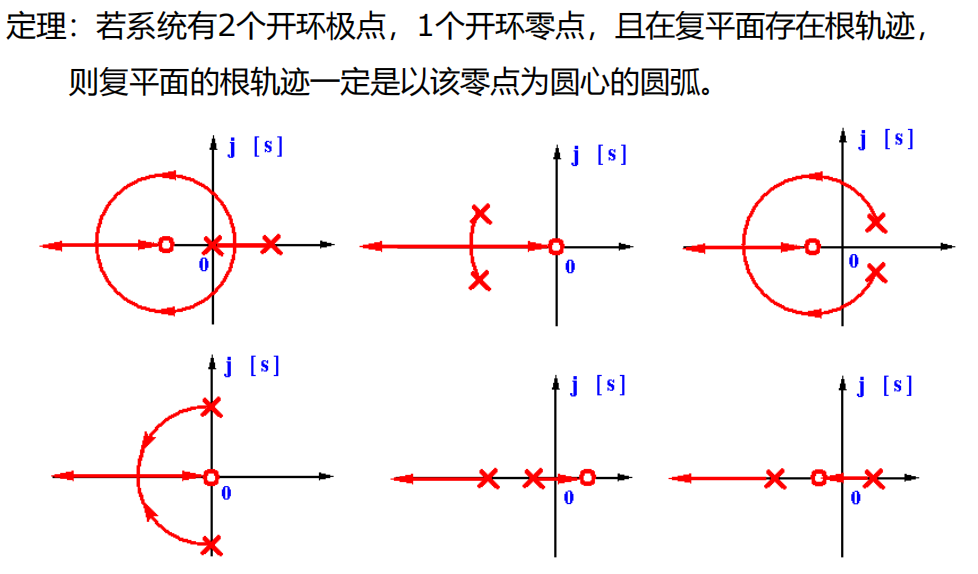
\includegraphics[width=\textwidth]{根轨迹圆弧.png}
                \caption{圆弧根轨迹定理}
            \end{subfigure}
            \hfill
            \begin{subfigure}[b]{0.48\textwidth}
                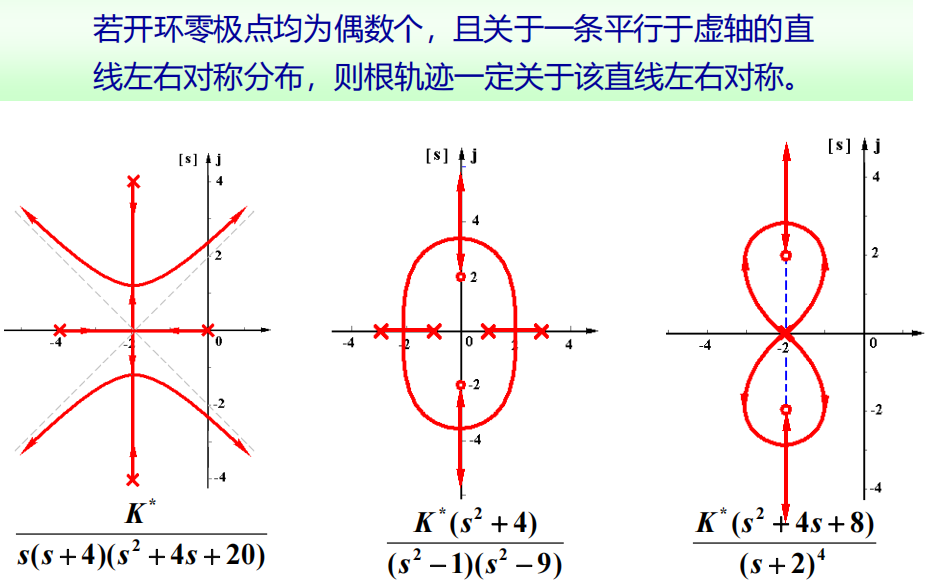
\includegraphics[width=\textwidth]{根轨迹对称性.png}
                \caption{根轨迹对称性定理}
            \end{subfigure}            
        \end{figure}
    \subsection{根轨迹分析系统性能}
        根据根轨迹确定系统稳定性对应的参数范围，根据系统型别和极点确定系统的稳态误差。根据幅值条件确定系统的参数，计算系统的动态性能。
    \subsection{特殊根轨迹}
        \subsubsection{正反馈系统的根轨迹（零度根轨迹）}
            \begin{itemize}
                \item 幅值条件：$|G(s)H(s)|=1$
                \item 相角条件：$\angle G(s)H(s)=\pm2k\pi$
            \end{itemize}

            因此，修改常规根轨迹法则中关于相角条件的部分：

            \begin{itemize}
                \item 规则3：对于实轴上的线段，若右侧的开环零极点数目之和为偶数，则该线段存在根轨迹。
                \item 规则4：相位角为$\varphi_a=\pm\dfrac{2k\pi}{n-m}$
                \item 规则7：$\sum\limits_{j=1}^m\angle (s-z_j)-\sum\limits_{i=1}^n\angle(s-p_i)=2k\pi$
            \end{itemize}
        \subsubsection{参数根轨迹}
            对于参变量$\lambda$，将特征方程写为$D(s)=Q(s)+\lambda P(s)=0$，等效传递函数$\bar G(s)\bar H(s)=\dfrac{\lambda P(s)}{Q(s)}$，则闭环极点与原系统相同，而闭环零点通常不同。
\newpage
\section{线性连续系统的频域分析}
    在正弦输入信号作用下，输出的稳态分量称为频率响应，频率响应与正弦输入信号的关系称为频率特性。

    将传递函数中的$s$以$\j\omega$代替得到频率特性$G(\j\omega)=|G(\j\omega)|\angle G(\j\omega)$，
    其中$|G(\j\omega)|$是输出与输入信号幅值之比，称为幅值特性；$\angle G(\j\omega)$是输出与输入信号相角之差，称为相频特性。

    对数幅频特性$L(\omega)=20\lg|G(\j\omega)|$，对数相频特性$\varphi(\omega)=\angle G(\j\omega)$。

    系统传递函数的极点和零点都在$s$平面左半平面的系统称为最小相位系统。对于幅频特性相同的系统，最小相位系统具有的相位滞后是最小的。最小相位系统的幅频特性对应唯一的相频特性。
    \subsection{控制系统的频率特性}
        \subsubsection{三种图形表示}
            奈奎斯特（Nyquist）图：以$|G(\j\omega)|$为极径，以$\angle G(\j\omega)$为极角绘制的极坐标频率特性图。

            伯德（Bode）图：以为对数幅频、相频特性为纵轴、以十倍频程为横轴绘制的对数坐标图。

            尼柯尔斯（Nichols）图：以对数幅频为纵轴、以相频为横轴并绘制等幅$M$线和等相$\alpha$线的半对数坐标图。
        \subsubsection{典型环节的频率特性}
            比例环节：$G(s)=K\begin{cases}L(\omega)=20\lg K\\\varphi(\omega)=0\end{cases}$

            惯性环节：$G(s)=\dfrac{1}{1+Ts}\begin{cases}L(\omega)=20\lg\sqrt{1+T^2\omega^2}\\\varphi(\omega)=-\arctan T\omega\end{cases}$

            积分环节：$G(s)=\dfrac{1}{s}\begin{cases}L(\omega)=-20\lg\omega\\\varphi(\omega)=-\dfrac{\pi}{2}\end{cases}$

            微分环节：$G(s)=s\begin{cases}L(\omega)=20\lg\omega\\\varphi(\omega)=\dfrac{\pi}{2}\end{cases}$

            一阶比例微分环节：$G(s)=1+Ts\begin{cases}L(\omega)=20\lg\sqrt{1+T^2\omega^2}\\\varphi(\omega)=\arctan T\omega\end{cases}$

            二阶微分环节：$G(s)=T^2s^2+2\zeta Ts+1\begin{cases}L(\omega)=20\lg\sqrt{(1-T^2\omega^2)^2+(2\zeta T\omega)^2}\\
            \varphi(\omega)=\begin{cases}\arctan(\dfrac{2\zeta T\omega}{1-T^2\omega^2})& \omega\leq\dfrac1T\\
            \pi-\arctan(\dfrac{2\zeta T\omega}{1-T^2\omega^2})&\omega>\dfrac1T\end{cases}\end{cases}$

            振荡环节：$G(s)=\dfrac{1}{T^2s^2+2\zeta Ts+1}\begin{cases}L(\omega)=-20\lg\sqrt{(1-T^2\omega^2)^2+(2\zeta T\omega)^2}\\
            \varphi(\omega)=\begin{cases}-\arctan(\dfrac{2\zeta T\omega}{1-T^2\omega^2})&\omega\leq\dfrac1T\\
            -\pi+\arctan(\dfrac{2\zeta T\omega}{1-T^2\omega^2})&\omega>\dfrac1T\end{cases}\end{cases}$

            延迟环节：$G(s)={\rm e}^{-\tau s}\begin{cases}L(\omega)=0\\\varphi(\omega)=-57.3^\circ\tau\omega\end{cases}$
            \begin{figure}[H]
                \centering
                \begin{subfigure}[b]{0.48\textwidth}
                    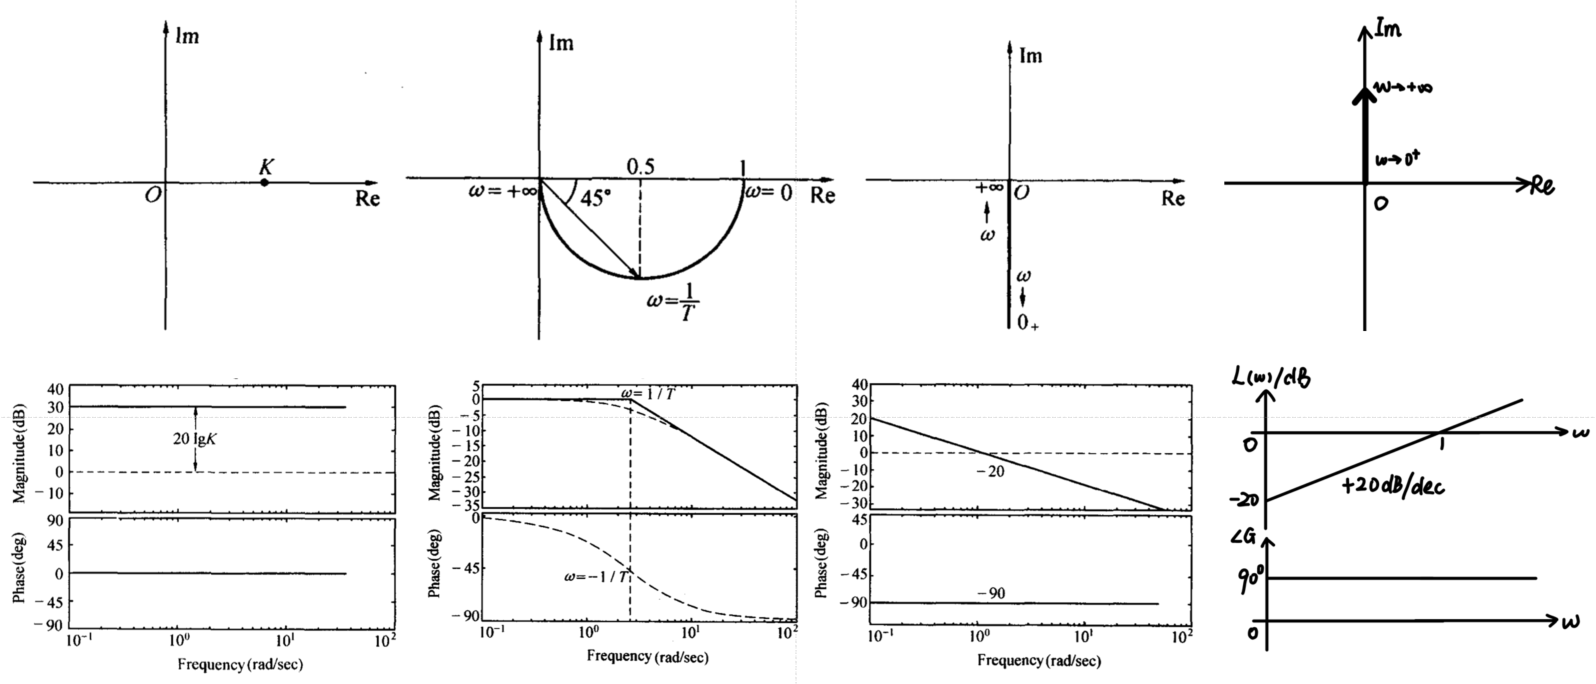
\includegraphics[width=\textwidth]{频率特性图1.png}
                    \caption{比例、惯性、积分、微分}
                \end{subfigure}
                \hfill
                \begin{subfigure}[b]{0.48\textwidth}
                    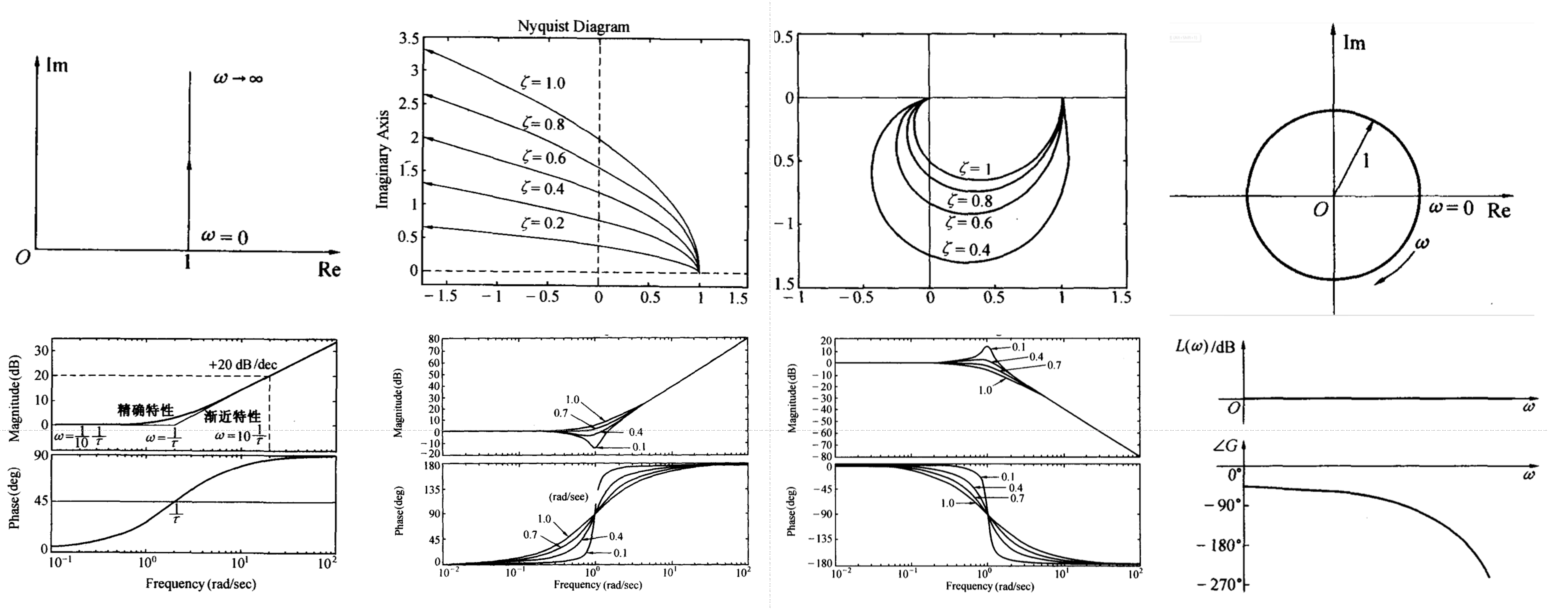
\includegraphics[width=\textwidth]{频率特性图2.png}
                    \caption{一阶微分、二阶微分、振荡、延迟}
                \end{subfigure}
            \end{figure}
        \subsubsection{系统开环频率特性绘制}
            最小相位系统Nyquist图的绘制：起点$\angle G(\j\omega)\rightarrow-90^\circ\cdot\nu$，若$n>m$终点在坐标原点，令${\rm Im}[G(\j\omega)]=0$求出与实轴交点，关注象限。
            \begin{figure}[H]
                \centering
                \begin{subfigure}[b]{0.32\textwidth}
                    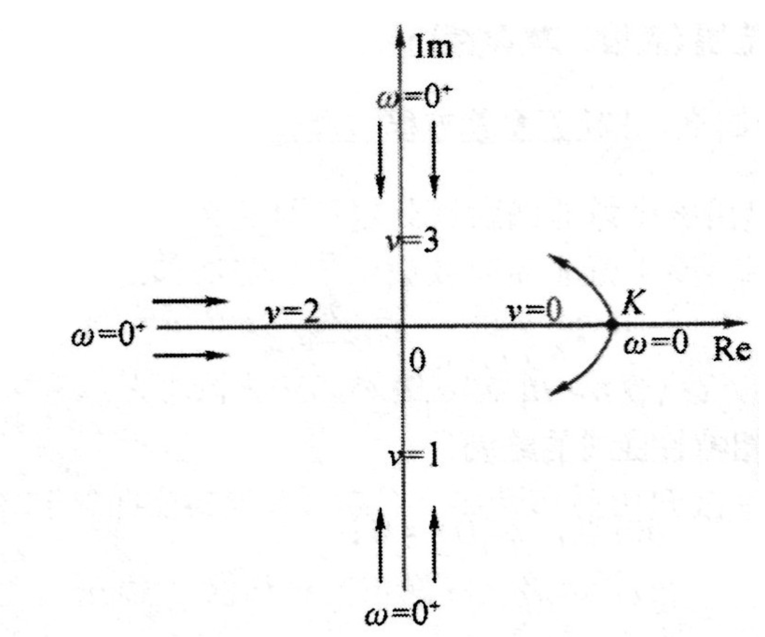
\includegraphics[width=\textwidth]{Nyquist起点.png}
                    \caption{Nyquist曲线起点}
                \end{subfigure}
                \begin{subfigure}[b]{0.32\textwidth}
                    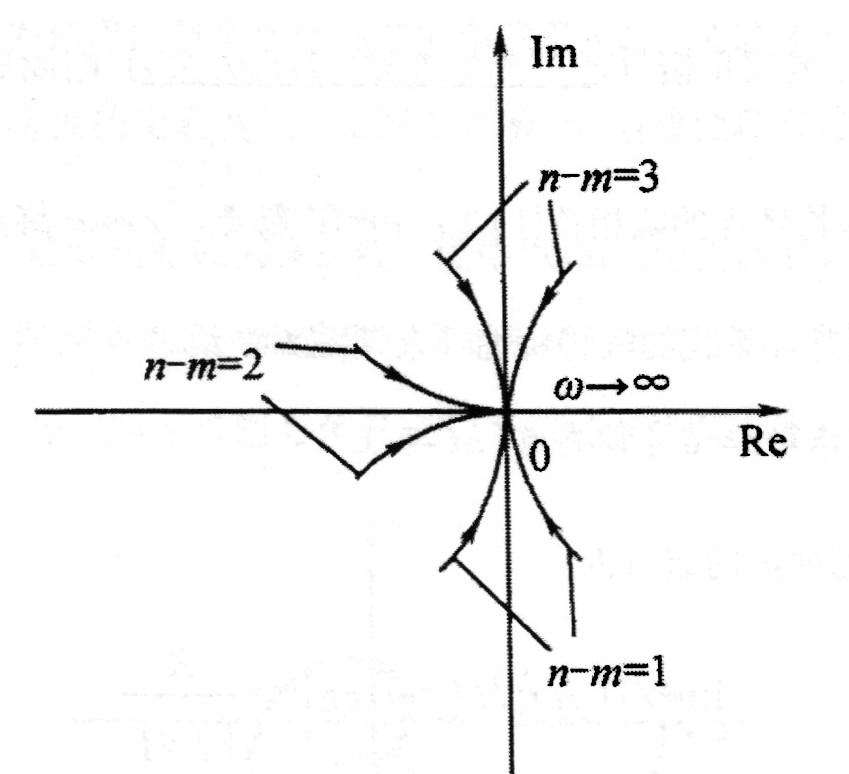
\includegraphics[width=\textwidth]{Nyquist终点.jpg}
                    \caption{Nyquist曲线终点}
                \end{subfigure}
            \end{figure}

            系统Bode图的绘制：$L(\omega)=\sum\limits_{i=1}^{n}L_i(\omega),\varphi(\omega)=\sum\limits_{i=1}^{n}\varphi_i(\omega)$，由各环节的Bode图相加得到。

            \begin{enumerate}
                \item 基准线：低频段的斜率为$-20\nu{\rm dB/dec}$，$\nu$为串联积分环节数，低频段或其延长线$\omega=1$处为$20\lg K$。
                \item 转折频率：一阶环节在$\dfrac{1}{T}$处斜率变化$\pm20{\rm dB/dec}$；二阶环节在$\omega_n$处斜率变化$\pm40{\rm dB/dec}$。
                \item 二阶环节修正：转折频率处为$\pm20\lg(2\zeta){\rm dB}$；谐振频率$\omega_r=\omega_n\sqrt{1-2\zeta^2}$处为$20\lg\dfrac{1}{2\zeta\sqrt{1-\zeta^2}}$。
            \end{enumerate}
    \subsection{闭环系统频域稳定性分析}        
        \subsubsection{奈奎斯特（Nyquist）稳定判据}
            \begin{minipage}{0.55\textwidth} % 文字区域（左侧）
                奈奎斯特回线：沿虚轴由下向上移动的直线段$C_1$和半径为无穷大的半圆$C_2$组成，包围右半平面所有的零极点。当$s$平面虚轴上存在开环极点时，奈奎斯特回线要从右边绕过无穷小半径的圆弧。

                沿虚轴$s=0$到$\infty$对应的映射为开环Nyquist曲线，无穷大的半圆对应的映射为原点，沿虚轴$s=-\infty$到$0$对应的映射与Nyquist曲线关于实轴对称，无穷小半径圆弧对应映射为无穷大半径的圆弧。
            \end{minipage}
            \hfill % 填充水平空间
            \begin{minipage}{0.4\textwidth} % 图片区域（右侧）
                \centering
                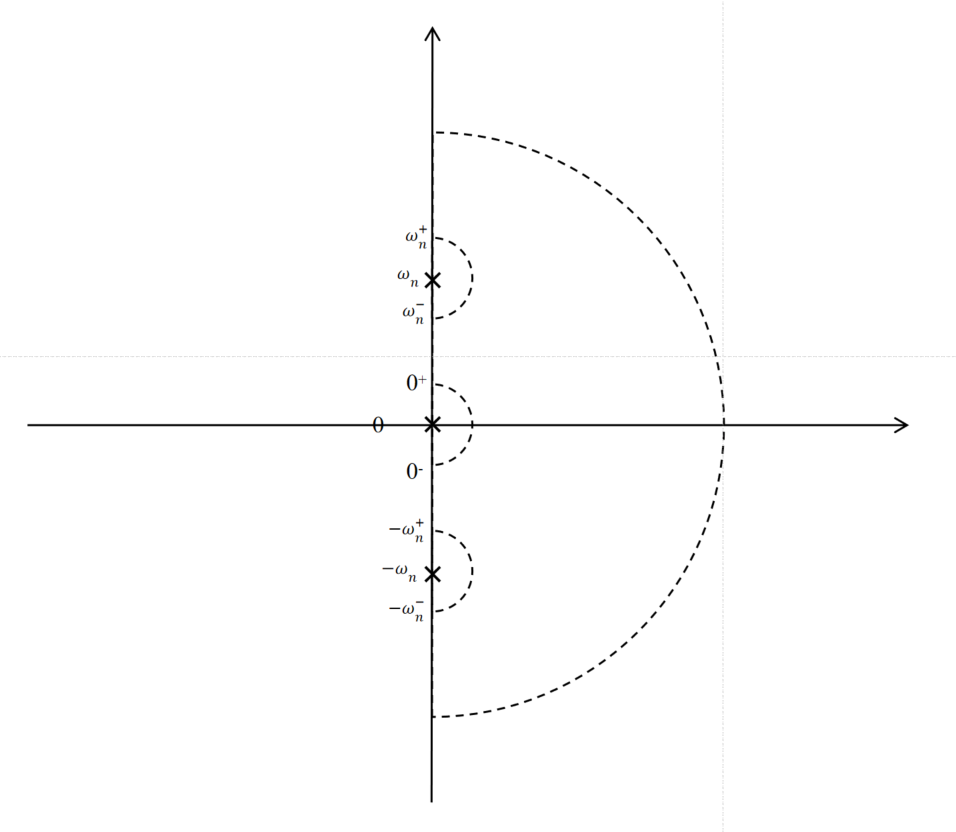
\includegraphics[width=\linewidth]{奈氏回线.png}
            \end{minipage}

            $Z=P-R=P-2N$，若$Z=0$，闭环系统稳定，若$Z>0$，闭环系统不稳定。
            其中$P$为右半平面开环极点个数，$R$为映射曲线包围$(-1,\j0)$点的圈数，$N$为开环Nyquist曲线包围$(-1,\j0)$点的圈数，$Z$为右半平面闭环极点个数。

            $N=N_+-N_-$，其中$N_+$为Nyquist曲线由上而下穿越次数，$N_-$为Nyquist曲线由下而上穿越次数。若起始或终止于$(-1,\j0)$点左侧的负实轴，则穿越次数为半次。
        \subsubsection{对数频率稳定判据}
            单位圆外对应$0{\rm dB}$以上的部分，单位圆内对应$0{\rm dB}$以下的部分。负实轴对应相频特性的$-180^\circ$线。
            当$s$平面虚轴上存在开环极点时，在对数相频曲线最低频率处，由下向上补画一条通过相角$\nu\cdot90^\circ$的曲线。

            $\varphi(\omega_c)\neq(2k+1)\pi$和$L(\omega)>0$时，若$Z=P-2N=0$，系统稳定。

            $N=N_+-N_-$，其中在$L(\omega)>0{\rm dB}$范围内，$N_+$为相频特性由下向上穿越$-180^\circ$次数，$N_-$为相频特性由上向下穿越$-180^\circ$次数。若起始或终止于$-180^\circ$线，则穿越次数为半次。
        \subsubsection{稳定裕度}
            在$L(\omega)=0$的剪切频率$\omega_c$下达到临界稳定所需滞后量称为相角裕度，$PM=\gamma=180^\circ+\varphi(\omega_c)$。
            在Bode图中，$\gamma$是对数相频曲线在$\omega_c$处与$-180^\circ$线的距离。
            对于具有两个或多个截止频率的系统，相角裕度应在最高的截止频率上测量。

            在$\varphi=-\pi$的穿越频率$\omega_g$处达到临界稳定所需增益量称为幅值裕度，$GM=K_g=\dfrac{1}{|G(\j\omega_g)H(\j\omega_g)|}$。
            在Bode图中，$-20\lg K_g$是对数幅频曲线在$\omega_g$处与$0{\rm dB}$线的距离。
            对于具有两个或多个穿越频率的系统，幅值裕度应在最高的穿越频率上测量。

            稳定裕度判据：对于最小相位系统，$\gamma>0$且$20\lg K_g>0$时，系统稳定。

            最小相位系统中，得到满意的响应一般需要$30^\circ<\gamma<60^\circ,K_g>6{\rm dB}$，且在幅值Bode图上穿越剪切频率的斜率需大于$-40{\rm dB/dec}$。
        \subsubsection{稳态误差}
            \begin{itemize}
                \item 最低频段是水平线则为0型系统，水平线高度为$20\lg K_p$
                \item 最低频段斜率为$-20{\rm dB/dec}$则为I型系统，最低频段在$\omega=1$处为$20\lg K_v$，与横轴交点$\omega_0=K_v$
                \item 最低频段斜率为$-40{\rm dB/dec}$则为II型系统，最低频段在$\omega=1$处为$20\lg K_a$，与横轴交点$\omega_0=\sqrt{K_a}$
            \end{itemize}
    \subsection{动态性能分析}
        {\setlength{\parindent}{15pt}\textbf{频域性能指标：}}
        \begin{itemize}
            \item 零频值：$\omega=0$时闭环幅频特性的值$M_0$。
            \item 谐振峰：幅频特性的最大值与零频幅值之比$M_r=\dfrac{\max\ A(\omega)}{A(0)}$。
            \item 谐振频率：谐振峰对应的频率，$A(\omega_r)=\max\ A(\omega)$。
            \item 带宽频率：当频率特性的幅值下降到$1/\sqrt2$时对应的频率，$\sqrt2A(\omega_b)=A(0)$。
        \end{itemize}

        \textbf{对于二阶系统：}

        $M_0=1,\omega_r=\omega_n\sqrt{1-2\zeta^2},M_r=\dfrac{1}{2\zeta\sqrt{1-\zeta^2}},\omega_b=\omega_n\sqrt{1-2\zeta^2+\sqrt{2-4\zeta^2+4\zeta^4}}$

        $\omega_c=\omega_n\sqrt{\sqrt{4\zeta^4+1}-2\zeta^2},\gamma=\arctan\dfrac{2\zeta}{\sqrt{\sqrt{4\zeta^4+1}-2\zeta^2}}$

        \textbf{对于高阶系统，有经验公式：}

        $\sigma\%=0.16+0.4(\dfrac{1}{\sin\gamma}-1),34^\circ<\gamma<90^\circ,1\leqslant M_r\leqslant1.8$

        $t_s=\dfrac{\pi}{\omega_c}[2+1.5(\dfrac{1}{\sin\gamma}-1)+2.5(\dfrac{1}{\sin\gamma}-1)^2],34^\circ<\gamma<90^\circ,1\leqslant M_r\leqslant1.8$
        
        谐振频率出现在剪切频率附近，$\omega_r\approx\omega_c$，则$M_r=M_{max}/M_0\approx\dfrac{1}{\sin\gamma}$

        \textbf{闭环频域指标和时域指标的关系：}
        
        $\sigma\%=0.41\ln\bigg(\dfrac{M_rM(\frac{\omega_0}{4})\omega_b}{M_0^2\omega_{0.5}}\bigg)+0.17$

        $t_s=(13.6\dfrac{M_r\omega_b}{M_0\omega_{0.5}}-2.51)\dfrac{1}{\omega_{0.5}}$
\newpage
\section{线性连续系统的校正}
    校正：在系统中引入一些附加装置用来校正系统的暂态和稳态性能，使其全面满足性能指标要求。

    设计校正装置的过程：
    \begin{enumerate}
        \item 已知系统固有部分结构、特性和参量，绘制固有部分开环Bode图；
        \item 列出需要满足的性能指标；
        \item 从性能指标要求确定期望特性，绘制期望特性Bode图；
        \item 验算设计装置是否满足指标要求，若不满足需要重新设计。
    \end{enumerate}
    \subsection{PID控制律}
        \subsubsection{各控制器的作用}
            P控制器：$G_c(s)=K_P$，则$G(s)=G_c(s)G_o(s)=K_PG_o(s)$
            P控制下闭环极点沿根轨迹移动，$K_P$增加，稳态误差减小，与此同时系统超调增大，振荡加剧，影响稳定性。

            PD控制器：$G_c(s)=K_P+K_Ds$，则$G(s)=G_c(s)G_o(s)=(K_P+K_Ds)G_o(s)$，相当于增加一个零点$-\dfrac{K_P}{K_D}$，
            PD控制下随着D控制作用的加强，根轨迹向左移动。$K_D$增加，引入正相角提高相角裕度，提高稳定性。在$K_P$减小阻尼同时增大阻尼以减小超调和调节时间。减弱抗干扰性，放大高频干扰。实质是一种“预见性”控制。

            PI控制器：$G_c(s)=K_P+\dfrac{K_I}{s}$，则$G(s)=G_c(s)G_o(s)=\dfrac{K_Ps+K_I}{s}G_o(s)$，相当于增加极点$0$和零点$-\dfrac{K_I}{K_P}$，提高系统型别。
            使用I控制后，稳态误差主要靠提高型别调整，可以适当减小$K_P$的取值。$K_I$增加，提高系统精度，改善暂态响应，但是引入滞后相角对稳定性不利，一般需要$K_P>K_I$。

            PID控制器：$G_c(s)=K_P+\dfrac{K_I}{s}+K_Ds$，为系统增加极点$0$两个位于左半平面的零点，且提高系统型别，在提高性能方面具有很大的优越性。
        \subsubsection{PID整定}
            \textbf{齐格勒-尼科尔斯（Ziegler-Nichols）临界比例度法}

            调试方法：先将积分和微分增益设为0，比例增益从零开始增加到控制器输出等幅振荡，此时增益为极限增益$K_u$，振荡周期为$T_u$，根据下表确定PID参数。

            \begin{table}[H]
                \centering
                \begin{tabular}{|c|c|c|c|}
                \hline    
                    控制类型 & $K_P$ & $K_I$ & $K_D$ \\
                    \hline
                    P &  $0.5K_u$ &  & \\
                    \hline
                    PI &  $\dfrac{K_u}{2.2}$ & $\dfrac{1.2K_P}{T_u}$ & \\
                    \hline
                    PD &  $0.8K_u$ &  & $\dfrac{K_PT_u}{8}$ \\
                    \hline
                    PID &  $0.60K_u$ & $\dfrac{2K_P}{T_u}$ & $\dfrac{K_PT_u}{8}$ \\
                    \hline
                    Pessen Integral Rule &  $0.7K_u$ & $\dfrac{2.5K_P}{T_u}$ & $0.15K_PT_u$ \\
                    \hline
                    部分过冲量 &  $0.33K_u$ & $\dfrac{2K_P}{T_u}$ & $\dfrac{K_PT_u}{3}$ \\
                    \hline
                    无过冲量 &  $0.2K_u$ & $\dfrac{2K_P}{T_u}$ & $\dfrac{K_PT_u}{3}$ \\
                \hline
                \end{tabular}
            \end{table}
            
            \textbf{齐格勒-尼科尔斯（Ziegler-Nichols）阶跃响应法}
            
            \begin{minipage}{0.55\textwidth} % 文字区域（左侧）
                调试方法：系统没有积分环节和复数极点时，闭环阶跃响应曲线为$G(s)=\dfrac{K\e^{-\tau s}}{Ts+1}$，根据拐点切线和时间轴、和$c(t)=K$的交点得到$\tau$和$T$的值，根据下表确定PID参数。
            \end{minipage}
            \hfill % 填充水平空间
            \begin{minipage}{0.4\textwidth} % 图片区域（右侧）
                \centering
                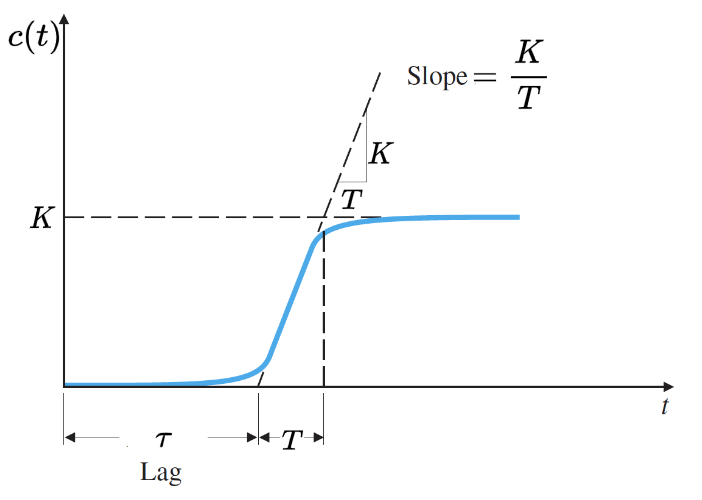
\includegraphics[width=0.6\linewidth]{Z-N阶跃响应法.png}
            \end{minipage}

            \begin{table}[H]
                \centering
                \begin{tabular}{|c|c|c|c|}
                \hline    
                    控制类型 & $K_P$ & $T_i$ & $T_d$ \\
                    \hline
                    P &  $\dfrac{T}{\tau}$ &  & \\
                    \hline
                    PI &  $\dfrac{0.9T}{\tau}$ & $\dfrac{\tau}{0.3}$ & \\
                    \hline
                    PID &  $\dfrac{1.2T}{\tau}$ & $2\tau$ & $0.5\tau$ \\
                \hline
                \end{tabular}
            \end{table}
    \subsection{串联校正}
        \subsubsection{串联超前校正}
            \begin{figure}[H]
                \centering
                \begin{subfigure}[b]{0.3\textwidth}
                    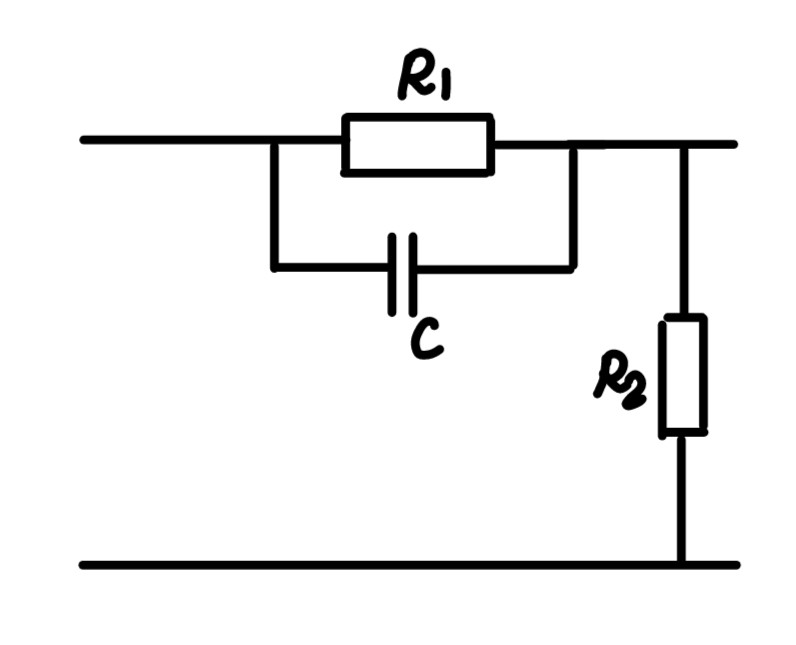
\includegraphics[width=\textwidth]{超前网络.jpg}
                    \caption{无源超前网络}
                \end{subfigure}
                \hfill
                \begin{subfigure}[b]{0.3\textwidth}
                    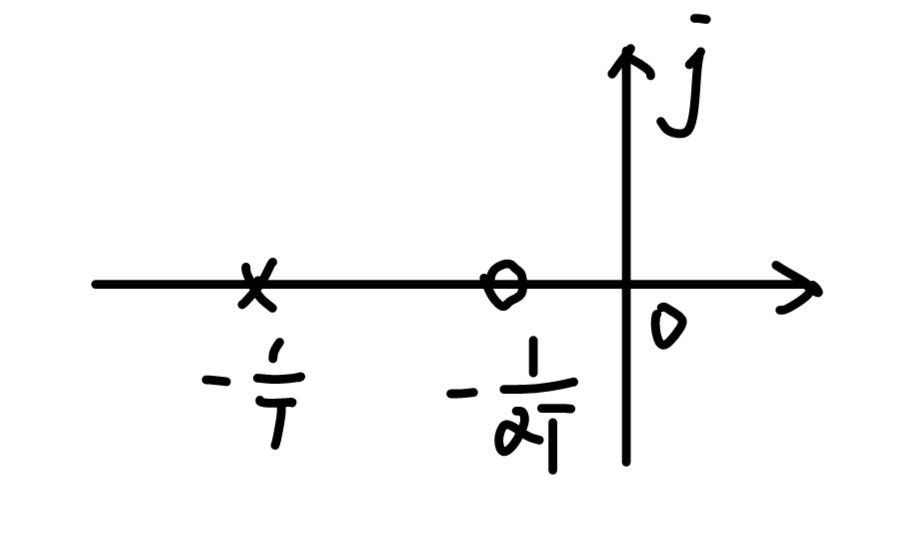
\includegraphics[width=\textwidth]{超前零极点分布.jpg}
                    \caption{超前网络零极点分布}
                \end{subfigure}
                \hfill
                \begin{subfigure}[b]{0.3\textwidth}
                    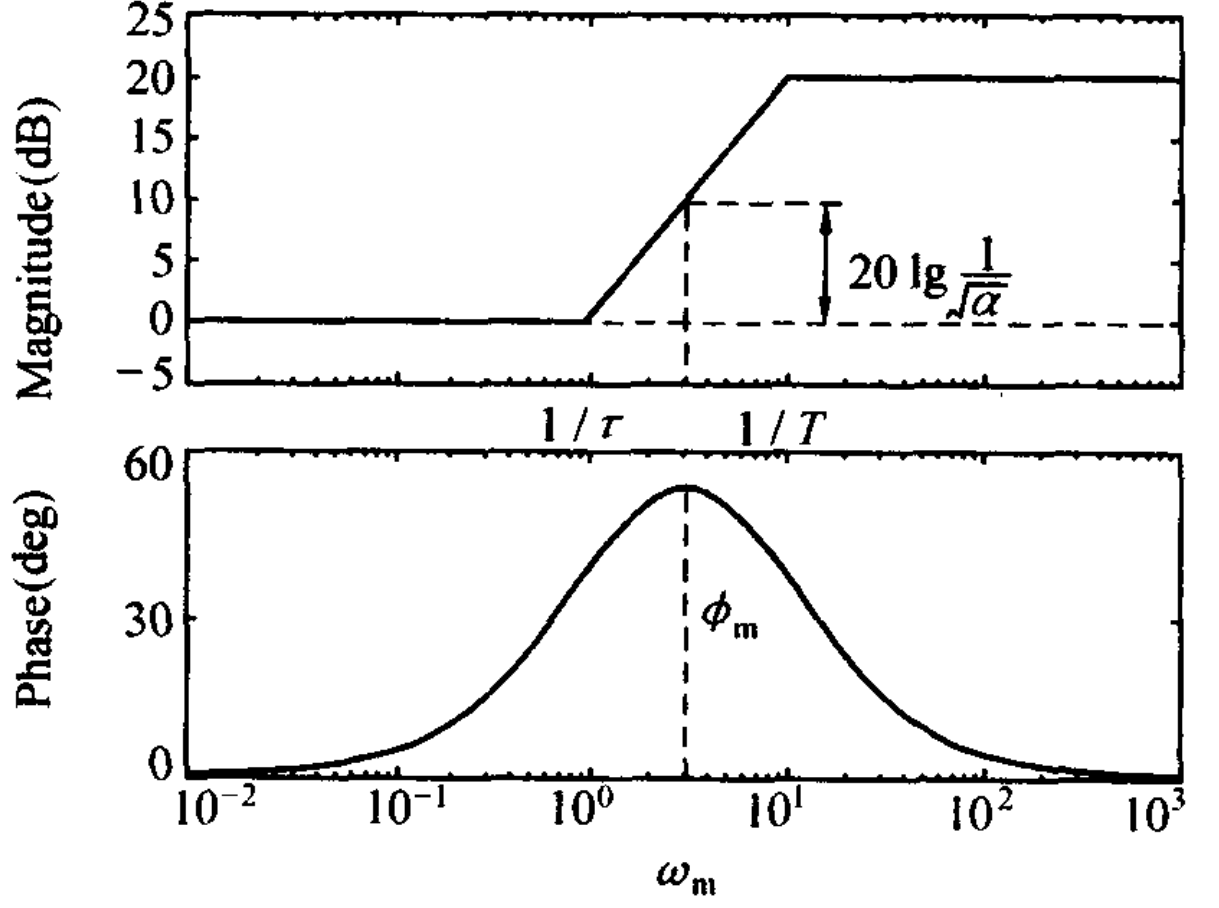
\includegraphics[width=\textwidth]{超前网络Bode.png}
                    \caption{超前网络Bode图}
                \end{subfigure}            
            \end{figure}
            
            $G_c(s)=\dfrac{R_2}{R_2+\frac{R_1}{1+sR_1C}}=\dfrac{\alpha Ts+1}{\alpha(Ts+1)}$，其中$\alpha=\dfrac{R_1+R_2}{R_2}>1,T=\dfrac{R_1R_2C}{R_1+R_2}$
            \begin{enumerate}
                \item 根据稳态误差要求，确定开环增益$K$；
                \item 绘制校正前Bode图，确定幅值和相角裕度$\gamma_0$；
                \item 确定最大相位超前角$\varphi_m=\gamma-\gamma_0+\varepsilon$，$\varepsilon=5^\circ\sim20^\circ$为考虑剪切频率处的负相角留出的裕度；
                \item 由$\alpha=\dfrac{1+\sin\varphi_m}{1-\sin\varphi_m}$确定超前网络的倍频比$\alpha$和对应角频率$\omega_m=\dfrac{1}{\sqrt\alpha T}$，此角频率为校正后的截止频率$\omega_c=\omega_m$；
                \item 确定转折频率$\omega_1=\dfrac{1}{T}=\omega_m\sqrt{\alpha},\omega_2=\dfrac{1}{\alpha T}=\dfrac{\omega_m}{\sqrt{\alpha}}$；
                \item 将原开环增益增加$\alpha$倍补偿超前网络产生的幅值衰减。
            \end{enumerate}

            超前网络相当于高通滤波器，提供正相角增大相角裕度，正幅值斜率增大幅值裕度，提高了快速性病改善了平稳性。但是$\alpha$的增大带来$L(\omega_m)=10\lg\alpha$的增加，降低了抗高频能力。
        \subsubsection{串联滞后校正}
            \begin{figure}[H]
                \centering
                \begin{subfigure}[b]{0.25\textwidth}
                    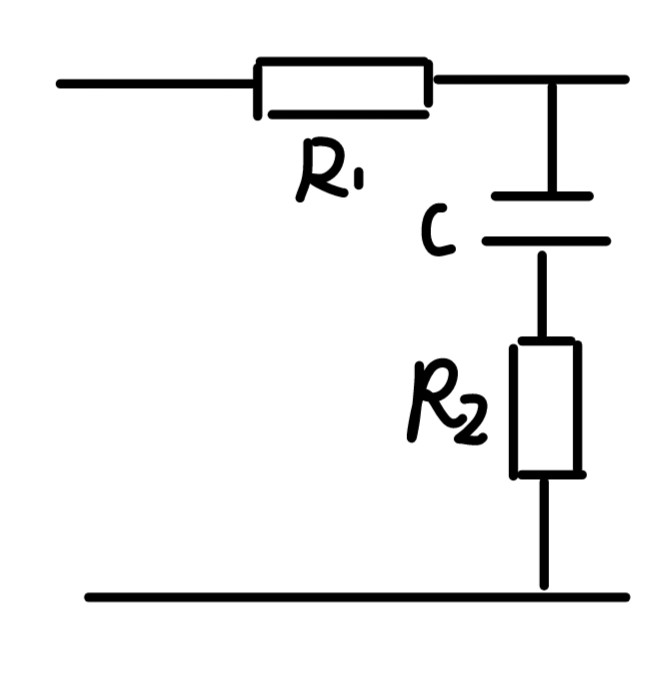
\includegraphics[width=\textwidth]{滞后网络.jpg}
                    \caption{无源滞后网络}
                \end{subfigure}
                \hfill
                \begin{subfigure}[b]{0.3\textwidth}
                    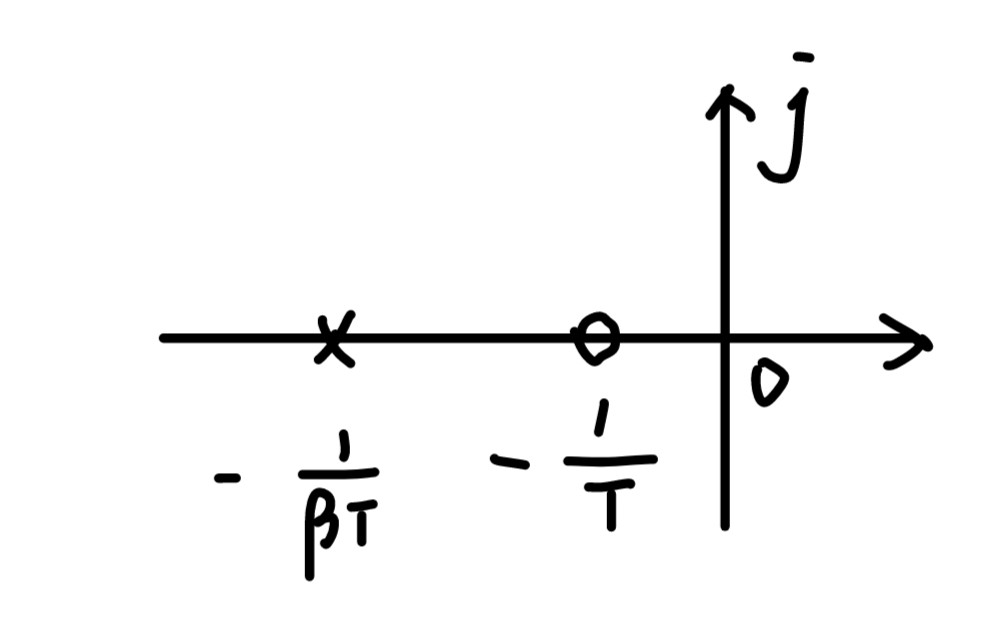
\includegraphics[width=\textwidth]{滞后零极点分布.jpg}
                    \caption{滞后网络零极点分布}
                \end{subfigure}
                \hfill
                \begin{subfigure}[b]{0.3\textwidth}
                    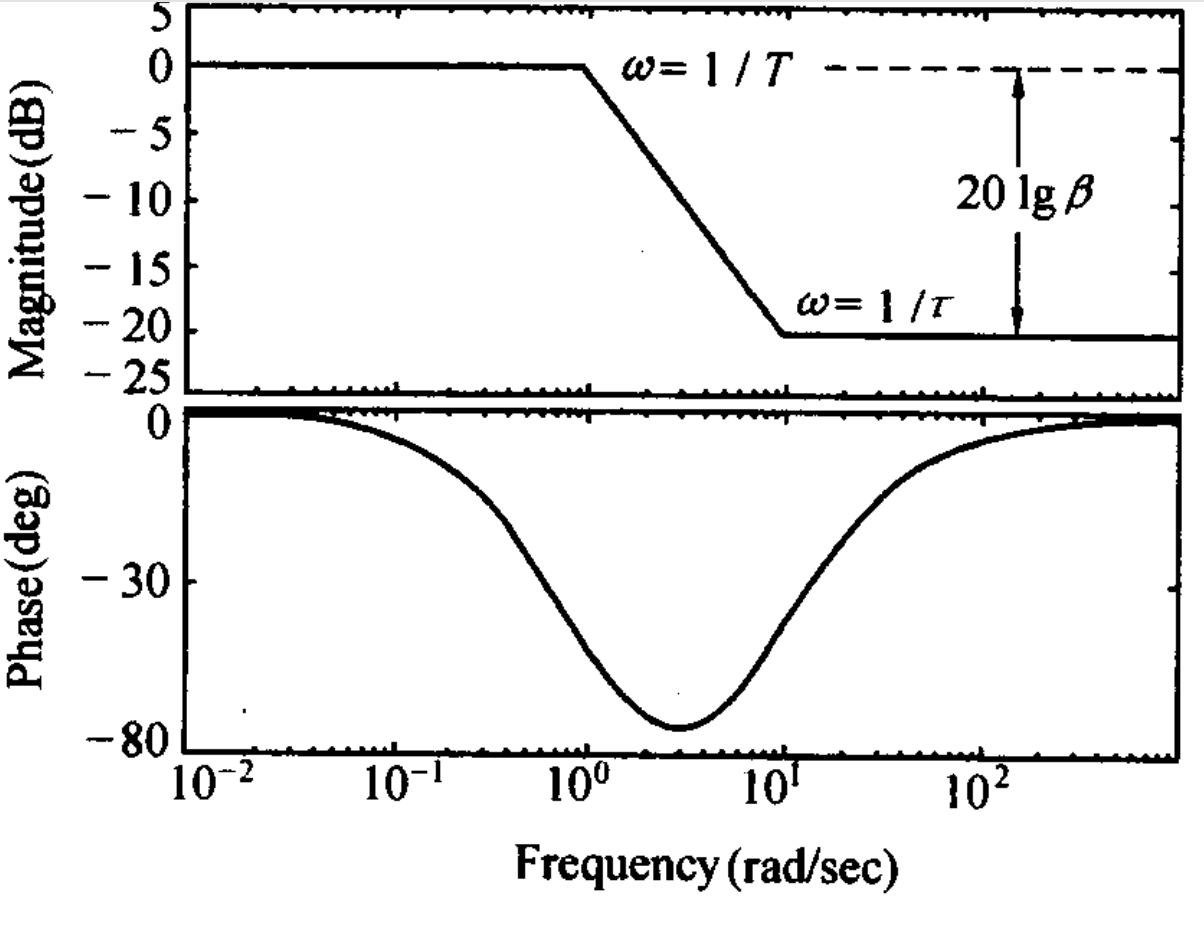
\includegraphics[width=\textwidth]{滞后网络Bode.png}
                    \caption{滞后网络Bode图}
                \end{subfigure}            
            \end{figure}
            
            $G_c(s)=\dfrac{R_2+\frac{1}{sC}}{R_1+R_2+\frac{1}{sC}}=\dfrac{\beta Ts+1}{Ts+1}$，其中$\beta=\dfrac{R_2}{R_1+R_2}<1,T=(R_1+R_2)C$
            \begin{enumerate}
                \item 根据稳态误差要求，确定开环增益$K$；
                \item 绘制校正前Bode图，确定幅值和相角裕度$\gamma_0$；
                \item 由$\varphi(\omega_c)=-180^\circ+\gamma+\varepsilon$确定校正后的截止频率，$\varphi_m=\arctan\dfrac{1-\beta}{2\sqrt\beta}$；
                \item 根据对数幅频曲线衰减到0所需衰减量为$-20\lg\beta$，确定$\beta$，再确定转折频率$\omega_2=\dfrac{1}{\beta T},\omega_1=\dfrac{1}{T}=\beta\omega_2$。
            \end{enumerate}

            滞后网络利用高频段的衰减加快中频段的下降，减小$\omega_c$，负幅值斜率压缩幅值从而调大开环增益，提高稳定精度和稳定裕量。但是频带变窄降低了快速性。
        \subsubsection{串联滞后-超前校正}
            \begin{figure}[H]
                \centering
                \begin{subfigure}[b]{0.3\textwidth}
                    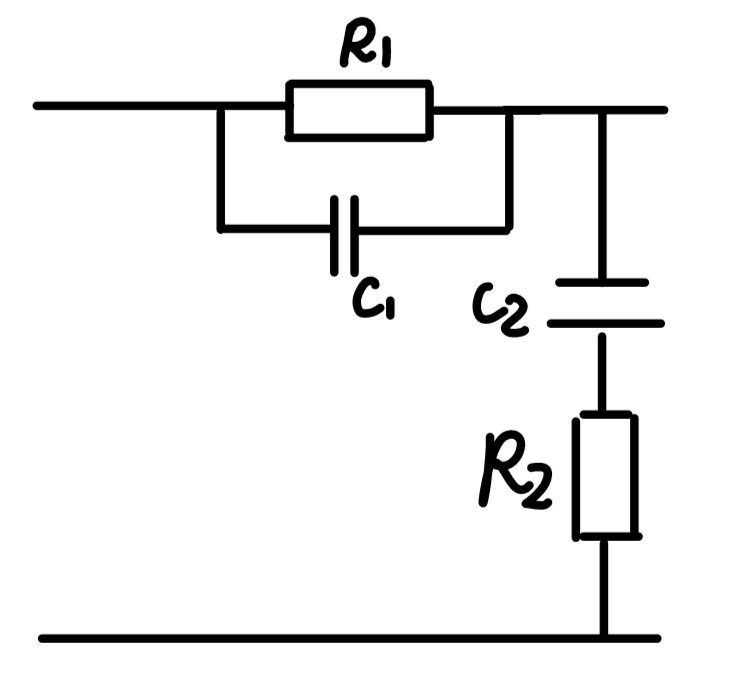
\includegraphics[width=\textwidth]{滞后超前网络.jpg}
                    \caption{无源滞后-超前网络}
                \end{subfigure}
                \hfill
                \begin{subfigure}[b]{0.3\textwidth}
                    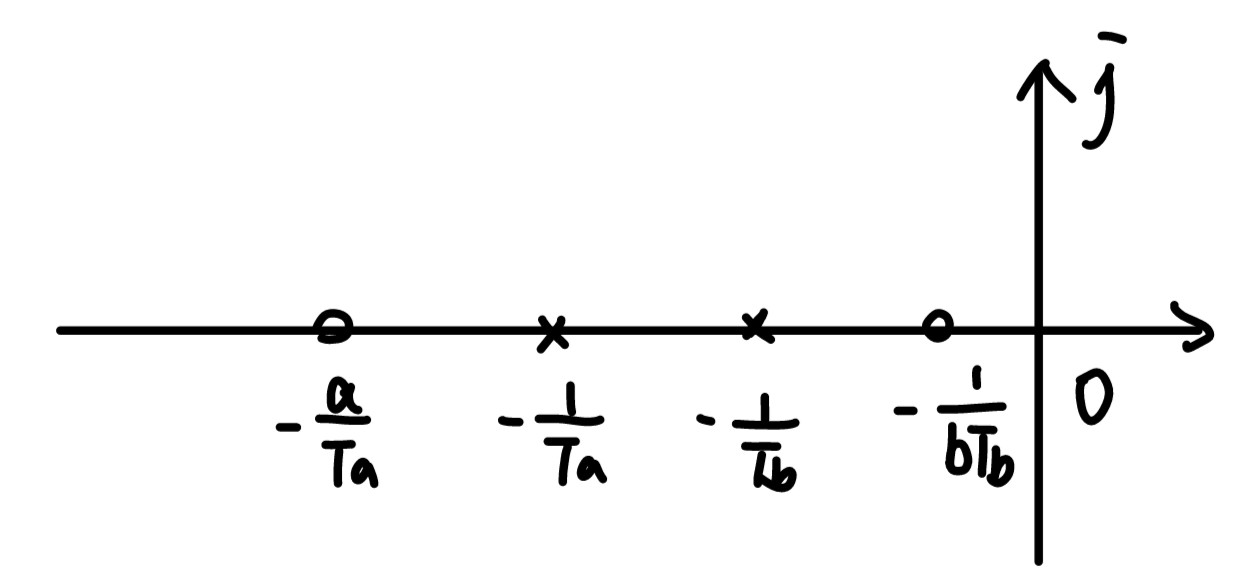
\includegraphics[width=\textwidth]{滞后超前零极点分布.jpg}
                    \caption{滞后-超前网络零极点分布}
                \end{subfigure}
                \hfill
                \begin{subfigure}[b]{0.3\textwidth}
                    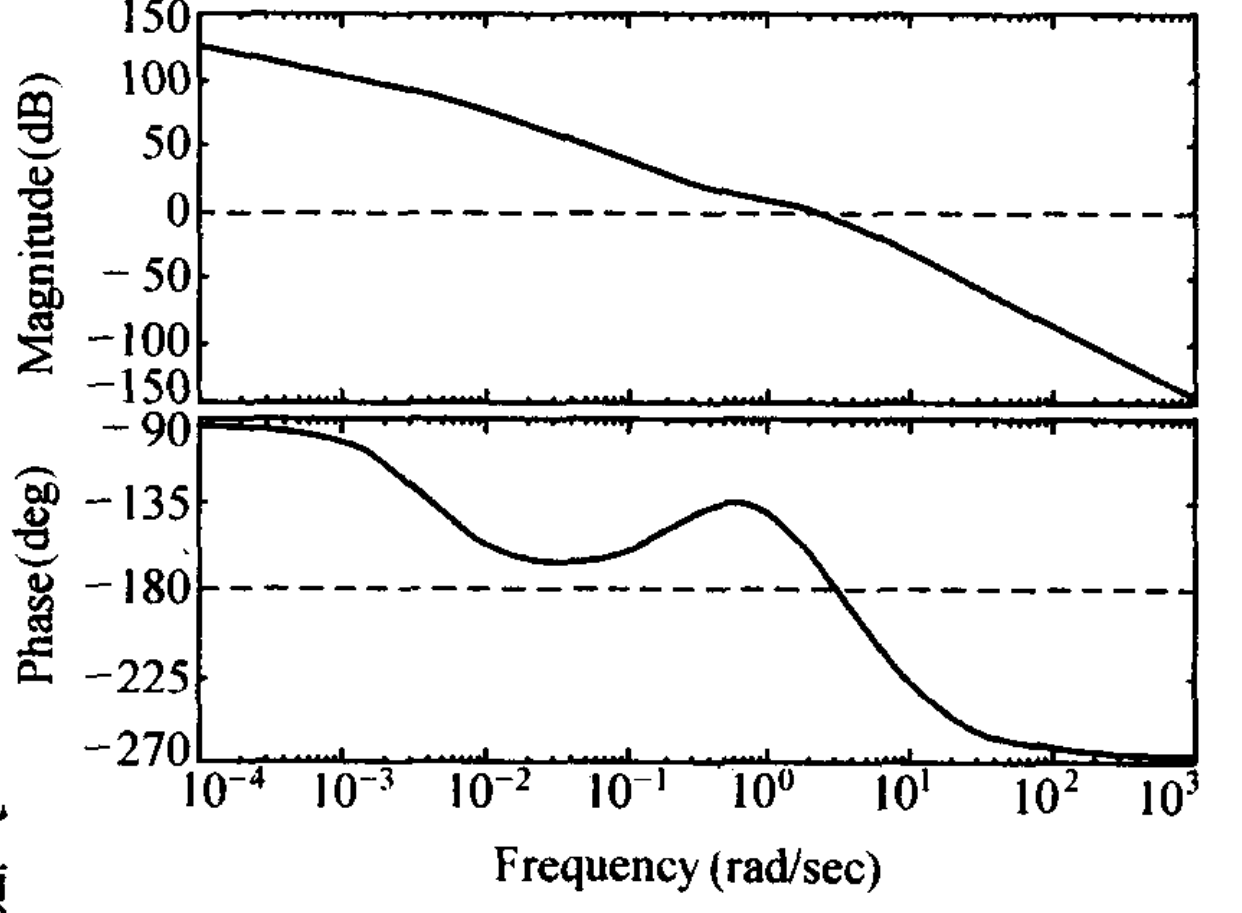
\includegraphics[width=\textwidth]{滞后超前网络Bode.png}
                    \caption{滞后-超前网络Bode图}
                \end{subfigure}            
            \end{figure}

            $G_c(s)=\dfrac{s+\frac{1}{T_b}}{s+\frac{1}{bT_b}}\dfrac{s+\frac{1}{T_a}}{s+\frac{a}{T_a}}$，其中$ab=1$
            \begin{enumerate}
                \item 根据稳态误差要求，确定开环增益$K$；
                \item 绘制校正前Bode图，确定幅值和相角裕度$\gamma_0$；
                \item 一般以校正前相角为$-180^\circ$对应的频率为校正后的$\omega_c$；
                \item 确定超前部分传递函数，由$-20\lg a+20\lg|G(\j\omega_c)|+20\lg T_B\omega_c=0$确定$a$，
                然后确定转折频率$\omega_{a1}=\dfrac{1}{T_b}=\dfrac{\omega_c}{\sqrt{a}},\omega_{a2}=\dfrac{a}{T_a}=a\omega_c$，
                则超前部分$G_{c1}(s)=\dfrac{T_as+1}{(T_a/a)s+1}$；
                \item 滞后部分转折频率$\omega_{b1}=\dfrac{1}{T_b}=(0.1\sim0.25)\omega_c,\omega_{b2}=\dfrac{1}{aT_b}$，滞后部分$G_{c2}(s)=\dfrac{T_bs+1}{aT_bs+1}$。
            \end{enumerate}
            
            将滞后效应设置在低频段，超前效应设定在中频段，确保效应优势充分发挥，提高系统动态性能和精度。
    \subsection{反馈校正}
        通过引入局部反馈，以局部反馈的零极点代替原局部的零极点，改变局部参数，消除不希望折点。
        \begin{figure}[H]
            \centering
            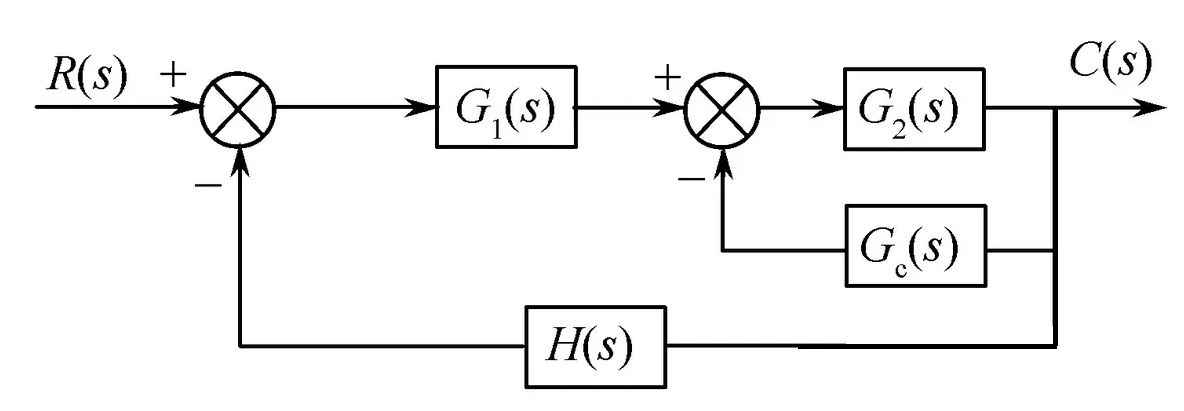
\includegraphics[width=8cm]{反馈校正.png}
            \caption{反馈校正}
        \end{figure}
        \begin{enumerate}
            \item 绘制开环幅频特性$L_0(\omega)$和期望开环幅频特性$L(\omega)$；
            \item 求得传递函数$20\lg|G_2(\j\omega)G_c(\j\omega)|=L_0(\omega)-L(\omega)$；
            \item 检验局部反馈的稳定性和剪切频率附近$|G_2(\j\omega)G_c(\j\omega)|>1$的程度；
            \item $G_c(s)=\dfrac{G_2(s)G_c(s)}{G(s)}$。
        \end{enumerate}

        与串联校正相比，反馈校正具有削弱非线性因素影响、对模型摄动不敏感、对干扰有抑制作用等特点，但是由于需要引入测量部件提高了系统的成本，且由于反馈对系统影响复杂，设计调整较为麻烦。

        深度反馈：若内环稳定且$|G_2(\j\omega)H(\j\omega)|>>1$，则$G_{2c}(\j\omega)=\dfrac{1}{H(\j\omega)}$，则反馈校正装置可以完全替代被包围环节，消除不希望的特性，抑制$G_2(s)$参数变化和干扰的影响。
    \subsection{复合校正}
        在系统中加入一个前馈通路，组成一个前馈校正和其他校正相结合的系统，不但可以保持系统的稳定性，还可以极大减少甚至消除稳态误差。

        \begin{figure}[H]
            \centering
            \begin{subfigure}[b]{0.48\textwidth}
                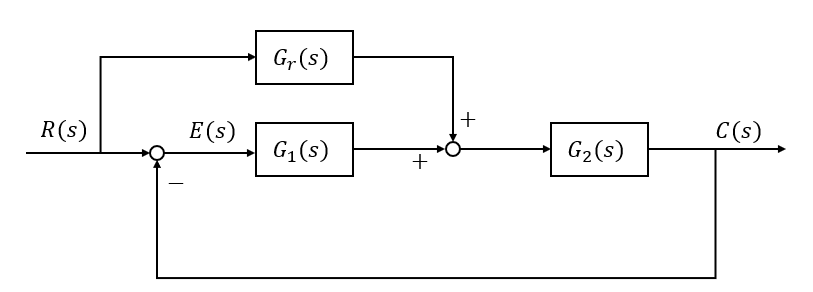
\includegraphics[width=\textwidth]{输入补偿.png}
                \caption{按输入端的复合校正}
            \end{subfigure}
            \begin{subfigure}[b]{0.48\textwidth}
                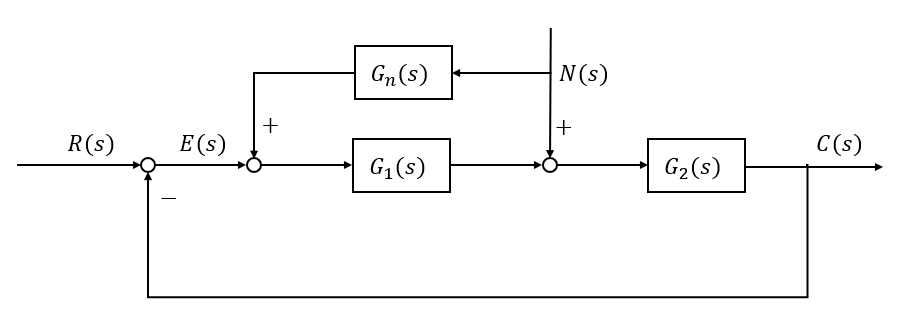
\includegraphics[width=\textwidth]{扰动补偿.png}
                \caption{按扰动的复合校正}
            \end{subfigure}  
        \end{figure}
        按输入端的复合校正：$E(s)=\dfrac{1-G_r(s)G_2(s)}{1+G_1(s)G_2(s)}R(s)$，因此令$G_r(s)=\dfrac{1}{G_2(s)}$则消除稳态误差，称为输入信号的误差全补偿条件。

        按扰动的复合校正：$E(s)=-\dfrac{G_2(s)[1+G_1(s)G_n(s)]}{1+G_1(s)G_2(s)}N(s)$，因此令$G_n(s)=\dfrac{1}{G_1(s)}$则消除稳态误差，称为扰动对误差全补偿条件。
\newpage
\section{线性离散系统的分析与校正}
    离散系统：在系统中有一处或几处信号是脉冲串或数码的系统。

    根据数值的连续性，离散系统分为：采样系统（数值连续） or 数字系统（数值量化）。
    \subsection{信号的采样与保持}
        \subsubsection{采样}
            A/D 过程用理想采样开关表示，采样时间为无穷小。即冲激函数采样，理想采样序列$\delta_T(t)=\sum\limits_{n=-\infty}^{\infty}\delta(t-nT)$

            采样过程：$e^*(t)=e(t)\cdot\delta_T(t)=\sum\limits_{n=0}^{\infty}e(nT)\delta(t-nT)$，$E^*(s)=\mathscr{L}[e^*(t)]=\sum\limits_{n=0}^{\infty}e(nT)\e^{-nTs}$

            将理想采样序列进行傅里叶级数展开：$\delta_T(t)=\dfrac{1}{T}\sum\limits_{n=-\infty}^{\infty}\e^{\j n\omega_st}$，
            则$E^*(s)=\mathscr{L}[e^*(t)]=\dfrac1T\sum\limits_{n=\infty}^{\infty}E(s+\j n\omega_s)$
    
            \begin{itemize}
                \item 时域表达式给出了$E^*(s)$和$e(t)$在采样点取值的关系，一般可写成封闭形式，用于求Z变换或时间响应。
                \item 傅里叶级数表达式给出了$E^*(s)$和$E(s)$的关系，一般不可以写成封闭形式，用于频谱分析。
            \end{itemize}
                
            香农（Shannon）采样定理：$\omega_s=\dfrac{2\pi}{T}>2\omega_h$或$T<\dfrac{\pi}{\omega_h}$，$\omega_h$为频谱带宽。
        \subsubsection{保持}
            D/A过程用零阶保持器（ZOH）表示，$k(t)=u(t)-u(t-T)$，
            
            因此$G_h(s)=\dfrac{1-\e^{-Ts}}{s}$，$G_h(\j\omega)=\dfrac{2\pi}{\omega_s}Sa(\pi\dfrac{\omega}{\omega_s})\e^{-j\pi\frac{\omega}{\omega_s}}$，
            相当于在系统中加入一个$\dfrac{T}{2}$的延迟环节。
    \subsection{数学模型}
        \subsubsection{差分方程}
            1阶前向差分：$\Delta e(k)=e(k+1)-e(k)$；1阶后向差分：$\nabla e(k)=e(k)-e(k-1)$

            n阶前向差分：$\Delta^ne(k)=\Delta^{n-1}e(k+1)-\Delta^{n-1} e(k)=e(k+n)+a_1^0e(k+n-1)+\cdots+a_{n-1}^0e(k+1)+a_n^0e(k)$
            
            n阶后向差分：$\nabla^ne(k)=\nabla^{n-1}e(k)-\nabla^{n-1} e(k-1)=e(k)+a_1^0e(k-1)+\cdots+a_{n-1}^0e(k-n+1)+a_n^0e(k-n)$
            
            n阶前向差分方程：
            $c(k+n)+a_1c(k+n-1)+a_2c(k+n-2)+\cdots+a_{n-1}c(k+1)+a_nc(k)=b_0r(k+m)+b_1r(k+m-1)+\cdots+b_{m-1}r(k+1)+b_mr(k)$

            n阶后向差分方程：
            $c(k)+a_1c(k-1)+a_2c(k-2)+\cdots+a_{n-1}c(k-n+1)+a_nc(k-n)=b_0r(k)+b_1r(k-1)+\cdots+b_{m-1}r(k-m+1)+b_mr(k-m)$ 
\newpage
        \subsubsection{Z变换}
            {\setlength{\parindent}{0pt}\textbf{6.2.1.1\quad Z正变换}}

            $E(z)=\mathscr{Z}[e^*(t)]=E^*(s)|_{z=\e^{Ts}}=\sum\limits_{n=0}^{\infty}e(nT)z^{-n}$
            
            \begin{figure}[H]
                \centering
                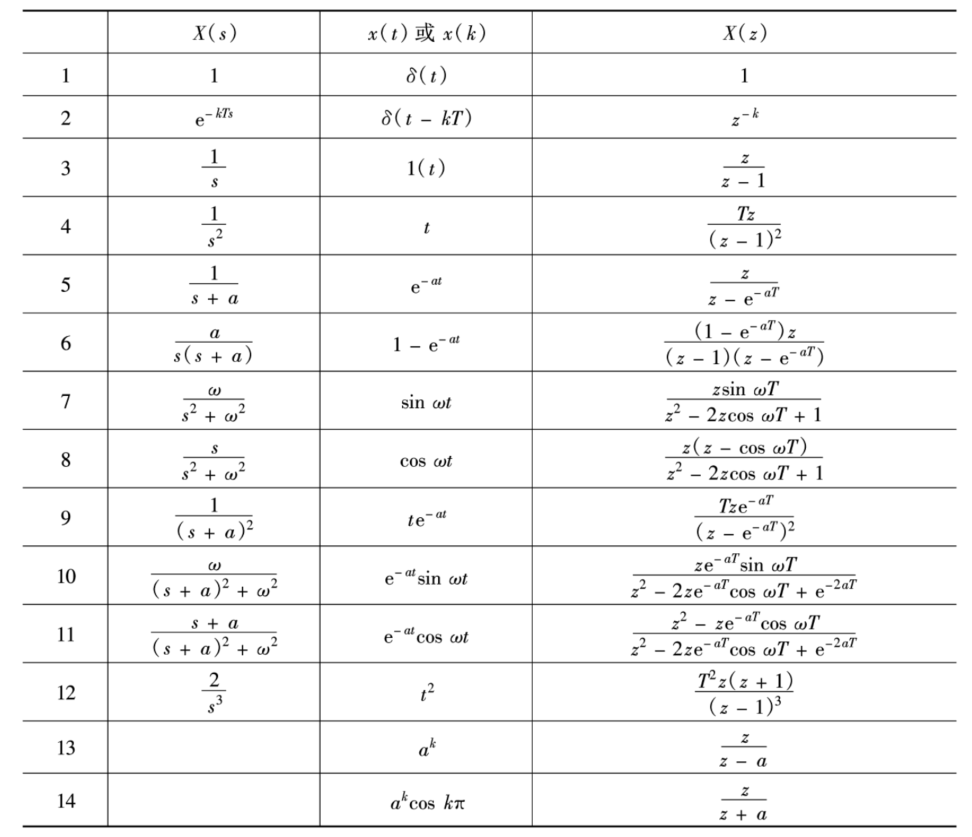
\includegraphics[width=8cm]{z变换公式表.png}
                \caption{Z变换表}
            \end{figure}

            留数积分法：$E(z)=\sum Res[E(s)\dfrac{z}{z-\e^{Ts}}]$

            {\setlength{\parindent}{0pt}\textbf{6.2.1.2\quad Z变换的性质}}

                \begin{enumerate}
                    \item 线性性质：$\mathscr{Z}[ae_1(t)+be_2(t)]=aE_1(z)+bE_2(z)$
                    \item 延迟性质：$\mathscr{Z}[e(t-nT)]=z^{-n}E(z)$      
                    \item 超前性质：$\mathscr{Z}[e(t+nT)]=z^n[E(z)-\sum\limits_{k=0}^{n-1}e(kT)z^{-k}]$        
                    \item 复位移性质：$\mathscr{Z}[e(t)\e^{\mp at}]=E(z\e^{\pm aT})$
                    \item 初值定理：$\lim\limits_{n\rightarrow0}e(nT)=\lim\limits_{z\rightarrow\infty}E(z)$        
                    \item 终值定理：$\lim\limits_{n\rightarrow\infty}e(nT)=\lim\limits_{z\rightarrow1}(z-1)E(z)$
                    \item 卷积定理：$\mathscr{Z}[e(t)*g(t)]=E(z)G(z)$
                \end{enumerate}

            {\setlength{\parindent}{0pt}\textbf{6.2.1.3\quad Z反变换}}
                
                \begin{enumerate}
                    \item 长除法：将真分式写成$z^{-1}$的升幂形式$\sum\limits_{n=1}^{\infty}a_nz^{-n}$，则$e(nT)=a_n$；
                    \item 对$\dfrac{E(z)}{z}$部分分式展开求出对应Z反变换；
                    \item 反演积分留数法：$e(nT)=\sum Res[E(z)z^{n-1}]$。
                \end{enumerate}
        \subsubsection{复数域数学模型}
            脉冲传递函数：零初始条件下离散系统输出Z变换与输入Z变换之比，即$G(z)=\dfrac{C(z)}{R(z)}$

            开环系统的脉冲传递函数：
            \begin{itemize}
                \item 环节之间有开关时，$G(z)=\mathscr{Z}[G_1(s)]\mathscr{Z}[G_2(s)]=G_1(z)G_2(z)$；
                \item 环节之间无开关时，$G(z)=\mathscr{Z}[G_1(s)G_2(s)]=G_1G_2(z)$；
                \item 有ZOH时，将ZOH视为$1$和$-\e^{-Ts}$的并联后经过一个理想开关后串联一个$\dfrac1s$，不改变系统的阶数，也不改变开环极点，只改变开环零点。
            \end{itemize}
            
            闭环系统的脉冲传递函数：$\varPhi(z)=\dfrac{G(z)}{1+GH(z)}$

            可用梅森增益公式的情况：
            (1)单回路无前馈通道离散系统，在前向通道存在至少一个实际的采样开关；
            (2)离散系统结构图中各环节之间均有或者等效有采样开关。
    \subsection{时域分析}
        \subsubsection{稳定性分析}
            {\setlength{\parindent}{0pt}\textbf{6.3.1.1\quad z域和s域的映射}}

            由于Z变换定义中$z=\e^{Ts}$，因此$z=\e^{(\sigma+\j\omega)T}=|z|\e^{\j\omega T}$，

            因此得到s平面和z平面的映射关系式：$|z|=\e^{\sigma T},\angle z=\omega T$。

            z平面的射线$Im[z]=\dfrac{\omega\pi }{\omega_s/2}Re[z]$映射为s平面的水平线$Im[s]=\omega$，

            z平面的圆$|z|=\e^\sigma$映射为s平面的垂直线$Re[s]=\sigma$。
            
            s平面左半部可以分成宽度为$\omega_s$频率范围为$\dfrac{2n-1}{2}\omega_s$到$\dfrac{2n+1}{2}\omega_s$的无数带域，每一个带域都映射为z平面的单位圆内的圆域，
            其中$-\dfrac{\omega_s}{2}$到$\dfrac{\omega_s}{2}$区域为主频带，其余为次频带。
            
            稳定的充要条件：所有特征根的模小于1，$|z_i|<1$，或者说全部特征根$z_i$都分布在z平面单位圆之内。

            {\setlength{\parindent}{0pt}\textbf{6.3.1.2\quad w域的劳斯（Routh）判据}}

            w变换：$z=\dfrac{w+1}{w-1}$，即$w=\dfrac{z+1}{z-1}$，是一个双线性变换。

            令$z=x+\j y$，则$w=\dfrac{x+1+\j y}{x-1+\j y}=\dfrac{x^2-1+y^2}{(x-1)^2+y^2}+\dfrac{-\j2y}{(x-1)^2+y^2}$

            故w平面虚轴是z平面的单位圆，即通过w变换将z平面的单位圆内区域映射为w平面的左半平面。

            在w平面内运用连续系统的劳斯（Routh）判据即可判定离散系统稳定性。

            {\setlength{\parindent}{0pt}\textbf{6.3.1.3\quad 朱利（Jurry）判据}}

            (1)$D(1)>0$；(2)$D(-1)\begin{cases}>0&n=2k\\<0&n=2k+1\end{cases}$；(3)$|a_0|<|a_n|$，$|b_0|>|b_{n-1}|$，$|c_0|>|c_{n-2}|$，$\cdots$
            \begin{table}[H]
                \centering
                \caption{朱利表}
                \begin{tabular}{c c c c c c}
                    $z^0$ & $z^1$ & $z^2$ & $\cdots$ & $z^{n-1}$ & $z^n$\\
                    $a_0$ & $a_1$ & $a_2$ & $\cdots$ & $a_{n-1}$ & $a_n$\\
                    $a_n$ & $a_{n-1}$ & $a_{n-2}$ & $\cdots$ & $a_1$ & $a_0$\\
                    $b_0$ & $b_1$ & $b_2$ & $\cdots$ & $b_{n-1}$ & \\
                    $b_{n-1}$ & $b_{n-2}$ & $b_{n-3}$ & $\cdots$ & $b_0$ & \\
                    $\vdots$ & $\vdots$ & $\vdots$ &  &  & \\
                    $q_0$ & $q_1$ & $q_2$ & & & \\
                \end{tabular}
            \end{table}

            朱利表共$2n+3$行。其中，第$2k+2$行各元是第$2k+1$行各元的反序排列。第一行元素为特征方程升幂排列的各项系数，
            从第三行起，$b_k=a_0a_k-a_{n-k}a_n,c_k=b_0b_k-b_{n-1}b_{n-k-1}$其余项以此类推

            {\setlength{\parindent}{0pt}\textbf{6.3.1.4\quad 舒尔-科恩（Schur-Cohn）判据}}

            \[
            \Delta_k=\begin{vmatrix}
                a_0 & 0 & 0 & \cdots & 0 & a_n & a_{n-1} & a_{n-2} & \cdots & a_{n-k+1} \\
                a_1 & a_0 & 0 & \cdots & 0 & 0 & a_n & a_{n-1} & \cdots & a_{n-k+2} \\
                a_2 & a_1 & a_0 & \cdots & 0 & 0 & 0 & a_n & \cdots & a_{n-k+3} \\
                \vdots & \vdots & \vdots &  & \vdots & \vdots & \vdots & \vdots &  & \vdots \\
                a_{k-1} & a_{k-2} & a_{k-3} & \cdots & a_0 & 0 & 0 & 0 & \cdots & a_n \\
                \bar a_n & 0 & 0 & \cdots & 0 & \bar a_0 & \bar a_1 & \bar a_2 & \cdots & \bar a_{k-1} \\
                \bar a_{n-1} & \bar a_n & 0 & \cdots & 0 & 0 & \bar a_0 & \bar a_1 & \cdots & \bar a_{k-2} \\
                \bar a_{n-2} & \bar a_{n-1} & \bar a_n & \cdots & 0 & 0 & 0 & \bar a_0 & \cdots & \bar a_{k-3} \\
                \vdots & \vdots & \vdots &  & \vdots & \vdots & \vdots & \vdots &  & \vdots \\
                \bar a_{n-k+1} & \bar a_{n-k+2} & \bar a_{n-k+3} & \cdots & \bar a_n & 0 & 0 & 0 & \cdots & \bar a_0 \\
            \end{vmatrix}_{2k}
            \]        

            规定$\Delta_0=1$条件下，各阶行列式按顺序$\Delta_0,\Delta_1,\Delta_2,\cdots,\Delta_n$的符号变更的数目就是稳定根的数目，如果多项式稳定，则变号次数等于多项式的次数。

            若$\Delta_k\begin{cases}<0&k=2n+1\\>0&k=2n\end{cases}$，则系统特征方程所有根都在单位圆内，此多项式称为舒尔（Schur）多项式。
        \subsubsection{动态性能分析}
            \begin{itemize}
                \item 实数极点：实轴上的极点$p_i$对应一个分量$y_i(kT)=B_ip_i^k$
                \begin{itemize}
                    \item 若$0<p_i<1$，极点在单位圆正实轴上，对应瞬态响应序列单调衰减；            
                    \item 若$p_i=1$，对应的是不变号的等幅序列；       
                    \item 若$p_i>1$，极点在单位圆外正实轴上，对应瞬态响应序列单调发散；                
                    \item 若$-1<p_i<0$，极点在单位圆内负实轴上，对应瞬态响应序列是正负号交替变号的衰减振荡序列；        
                    \item 若$p_i=-1$，对应瞬态响应是正负交替变号的等幅序列；
                    \item 若$p_i<-1$，极点在单位圆外负实轴上，对应瞬态响应序列是正负交替变号的发散序列。    
                \end{itemize}
                \item 共轭复数极点：$p_{i,i+1}=a\pm\j b$，对应的分量为$y_i(kT)=A_i\lambda_i^k\cos(k\theta_i+\phi_i)$，其中$\lambda_i=|p_i|,\theta_i=\arctan\frac{b}{a}$
                \begin{itemize}
                    \item 若$\lambda_i<1$，极点在单位圆内，对应的瞬态响应序列是收敛振荡的脉冲序列；
                    \item 若$\lambda_i=1$，极点在单位圆上，对应的瞬态响应序列是等幅振荡的脉冲序列；
                    \item 若$\lambda_i>1$，极点在单位圆外，对应的瞬态响应序列是发散振荡的脉冲序列。
                \end{itemize}
                
                其中，振荡角频率$\omega_i=\dfrac{\theta_i}{T}$，
                一个周期内包含的采样周期$N=\dfrac{\omega_s}{\omega_i}=\dfrac{2\pi}{\theta_i}$，
                当$\theta_i=\pi$时，对应频率最高的振荡，对系统损耗最大，因此尽量避免极点落在单位圆内负实轴上。    
            \end{itemize} 
            \begin{figure}[H]
                \centering
                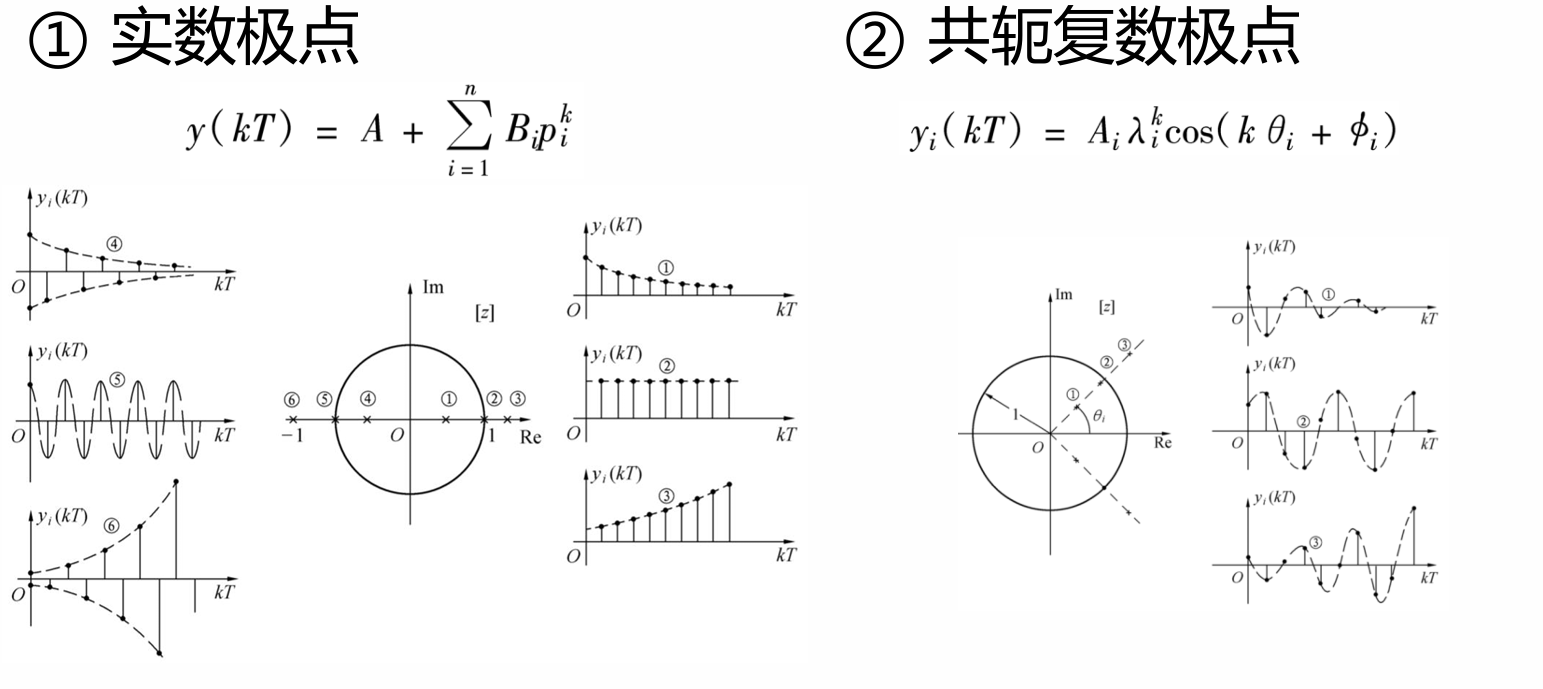
\includegraphics[width=0.8\textwidth]{离散极点.png}
                \caption{离散系统阶跃响应与极点的关系}              
            \end{figure}          
        \subsubsection{稳态误差}
            稳态误差$e^*_{ss}(t)$：过渡过程结束后再采样时刻系统希望输出与实际输出之差。

            稳态误差终值：$e^*_{ss}(\infty)=\lim\limits_{t\rightarrow\infty}e^*_{ss}(t)=\lim\limits_{t\rightarrow\infty}e^*(t)=\lim\limits_{z\rightarrow1}(z-1)E(z)$
            
            对单位负反馈系统，$\varPhi_e(z)=\dfrac{1}{1+G(Z)}$
            $e^*_{ss}(\infty)=\lim\limits_{t\rightarrow\infty}e^*_{ss}(t)=\lim\limits_{t\rightarrow\infty}e^*(t)=\lim\limits_{z\rightarrow1}(z-1)E(z)$
            把开环传递函数$G(z)$具有$z=1$极点的个数$\nu$作为划分离散系统型别的标准。

            单位阶跃响应，$e^*_{ss}(\infty)=\lim\limits_{z\rightarrow1}\dfrac{z}{1+G(z)}=\dfrac{1}{1+K_p}$，
            
            其中稳态位置误差系数$K_p:=\lim\limits_{z\rightarrow1}G(z)=\begin{cases}K&v=0\\\infty&v\geqslant1\end{cases}$

            单位斜坡响应，$e^*_{ss}(\infty)=\lim\limits_{z\rightarrow1}\dfrac{Tz}{(z-1)(1+G(z))}=\lim\limits_{s\rightarrow0}\dfrac{T}{(z-1)G(z)}=\dfrac{T}{K_v}$，
            
            其中稳态速度误差系数$K_v:=\lim\limits_{s\rightarrow0}(z-1)G(z)=\begin{cases}0&v=0\\K&v=1\\\infty&v=2\end{cases}$

            单位加速度响应，$e^*_{ss}(\infty)=\lim\limits_{z\rightarrow1}\dfrac{T^2z(z+1)}{2(z-1)^2(1+G(z))}=\lim\limits_{z\rightarrow1}\dfrac{T^2}{(z-1)^2G(z)}=\dfrac{T^2}{K_a}$，
           
            其中静态加速度误差系数$K_a:=\lim\limits_{z\rightarrow1}(z-1)^2G(z)=\begin{cases}0&v=0,1\\K&v=2\end{cases}$

            \begin{table}[H]
                \centering
                \caption{静态误差和型别的关系}
                \begin{tabular}{|c|c|c|c|c|c|c|}
                    \hline
                    型别 & $K_p$ & $K_v$ & $K_a$ & $r=A\cdot1(t)$ & $r=At$ & $r=A\frac{1}{2}t^2$\\
                    \hline
                    0 & $K$ & $0$ & $0$ & $\dfrac{A}{1+K}$ & $\infty$ & $\infty$ \\
                    \hline
                    I & $\infty$ & $K$ & $0$ & $0$ & $\dfrac{AT}{K}$ & $\infty$ \\
                    \hline
                    II & $\infty$ & $\infty$ & $K$ & $0$ & $0$ & $\dfrac{AT^2}{K}$ \\
                    \hline
                \end{tabular}
            \end{table}

            动态稳态误差系数：将$z=\e^{sT}$代入$\varPhi(z)$中得到$\varPhi_e(s)=\sum\limits_{m=0}^{\infty}\dfrac{1}{m!}\varPhi_e^{(m)}(s)s^m$。

            定义$c_m=\dfrac{1}{m!}\varPhi_e^{(m)}(s)$为动态稳态误差系数。
    \subsection{线性离散系统的校正}
        \subsubsection{模拟化设计}
            常用的离散化方法：
            \begin{itemize}
                \item 一阶差分近似法：$\dfrac{\d e}{\d t}\approx\dfrac{e(k)-e(k-1)}{T}$，则$D(z)=D(s)|_{s=\frac{1-z^{-1}}{T}}$\
                \item 阶跃响应不变法：串联一个虚拟的零阶保持器，$D(z)=\mathscr{Z}[\dfrac{1-\e^{-Ts}}{s}D(s)]$
                \item 根匹配法：$(s+a)\rightarrow(1-\e^{-aT}z^{-1}),(s+a\pm\j b)\rightarrow(1-2\e^{-aT}z^{-1}\cos bT+\e^{-2aT}z^{-2})$，若极点数大于零点数，其余极点为$(s+\infty)\rightarrow(z-0)$
                \item 双线性变换法：$s=\dfrac{1}{T}\ln z\approx\dfrac{2}{T}\dfrac{1-z^{-1}}{1+z^{-1}}$，$D(z)=D(s)|_{s=\frac{2}{T}\frac{1-z^{-1}}{1+z^{-1}}}$
                \item 脉冲响应不变法：$D(z)=\mathscr{Z}[D(s)]$
            \end{itemize}
        \subsubsection{最少拍系统的设计}
            采样过程的一个周期称为一拍。在典型输入信号作用下，经过最小采样周期，系统的采样误差减小到零实现完全跟踪，这样的系统称为最少拍系统，又称最快响应系统。

            串联数字校正系统的结构为输入信号$R(s)$经过理想采样开关后经过数字控制器$D(s)$，再经过理想采样开关后，经过$G(s)$得到$C(s)$。

            数字控制器脉冲传递函数$D(z)=\dfrac{\varPhi(z)}{G(z)[1-\varPhi(z)]}$或$D(z)=\dfrac{1-\varPhi_e(z)}{G(z)\varPhi_e(z)}$。

            典型输入信号$R(z)=\dfrac{A(z)}{(1-z^{-1})^\nu}$，误差$E(z)=R(z)\varPhi_e(z)$，
            则稳态误差为$e_{sr}=\lim\limits_{z\rightarrow1}(1-z^{-1})R(z)\varPhi_e(z)=\lim\limits_{z\rightarrow1}(1-z^{-1})\dfrac{A(z)}{(1-z^{-1})^\nu}\varPhi_e(z)$

            因此$\varPhi_e(z)=(1-z^{-1})^{\nu}F(z)$，则闭环脉冲传函$\varPhi(z)=1-(1-z^{-1})^\nu F(z)$，输出$C(z)R(z)\varPhi(z)=R(z)-A(z)F(z)$。

            显然当$F(z)=1$时，系统的暂态过程可以在最少拍内完成。则最少拍系统的闭环脉冲传函为$\varPhi(z)=1-(1-z^{-1})^\nu$，误差脉冲传函为$\varPhi_e(z)=(1-z^{-1})^\nu$。

            当$G(z)$包含单位圆外的零极点时，用$\varPhi_e(z)$的零点补偿$G(z)$在单位圆外的极点，用$\varPhi(z)$的零点补偿$G(z)$在单位圆外的零点，此时$F(z)\neq1$，而应补偿单位圆外的极点。

            最少拍系统暂态响应时间的增长和单位圆外的零极点个数成正比。

            最少拍系统的缺点：
            \begin{enumerate}
                \item 对不同输入信号适应性差；
                \item 对参数变化敏感，会延长暂态响应时间；
                \item 系统输出会出现波动，是有纹波系统。
            \end{enumerate}

            \begin{table}[H]
                \centering
                \caption{最少拍系统的校正}
                \begin{tabular}{|c|c|c|c|}
                    \hline
                    输入$r(t)$ & 误差脉冲传函$\varPhi_e(z)$ & 数字控制器$D(z)$ & 调整时间 \\
                    \hline
                    $1(t)$ & $1-z^{-1}$ & $\dfrac{z^{-1}}{(1-z^{-1})G(z)}$ & $T$ \\
                    \hline
                    $t$ & $(1-z^{-1})^2$ & $\dfrac{z^{-1}(2-z^{-1})}{(1-z^{-1})G(z)}$ & $2T$ \\
                    \hline
                    $\dfrac{1}{2}t^2$ & $(1-z^{-1})^3$ & $\dfrac{z^{-1}(3-3z^{-1}-z^{-2})}{(1-z^{-1})G(z)}$ & $3T$ \\
                    \hline
                \end{tabular}
            \end{table}
        \subsubsection{数字PID控制器设计}
            {\setlength{\parindent}{0pt}\textbf{全量型PID（位置型）}}    

            离散化得$m(k)=K_Pe(k)+TK_I\sum\limits_{j=0}^ke(j)+\dfrac{K_D}{T}[e(k)-e(k-1)]=K_pe(k)+K_i\sum\limits_{j=0}^ke(j)+K_d[e(k)-e(k-1)]$。
            
            其中$K_P,K_I,K_D$为模拟PID控制器的比例、积分、微分增益，
            
            $K_p=K_P,K_i=TK_I,K_d=\dfrac{K_D}{T}$为数字PID控制器的比例、微分、积分增益。

            求Z变换得脉冲传函为$G_c(z)=K_p+\dfrac{K_i}{1-z^{-1}}+K_d(1-z^{-1})=\dfrac{K_p(1-z^{-1})+K_i+K_d(1-z^{-1})^2}{1-z^{-1}}$.

            {\setlength{\parindent}{0pt}\textbf{增量型PID（速度型）}}

            对上式取差分得：$\Delta m(k)=m(k)-m(k-1)=(K_p+K_i+K_d)e(k)-(K_p+2K_d)e(k-1)+K_de(k-2)$，则$m(k)=m(k-1)+(K_p+K_i+K_d)e(k)-(K_p+2K_d)e(k-1)+K_de(k-2)$。
            
            求Z变换得脉冲传函$G_c(z)=\dfrac{(K_p+K_i+K_d)-(K_p+2K_d)z^{-1}+K_dz^{-2}}{1-z^{-1}}$，与全量型脉冲传函一致。

            增量型PID抗饱和能力强，切换输入时产生的冲击较小。
\newpage
\section{非线性系统分析}
    \subsection{非线性系统概述}
        非线性系统是指存在一个及以上非线性环节的系统，非线性系统缺乏线性和叠加性。
        \subsubsection{非线性系统的特点}
            \begin{enumerate}
                \item 具有多个平衡点，且系统稳定性除了与系统的结构形式和参数有关外，还和初始条件和外部输入有关。
                \item 除了状态发散或者收敛于平衡状态两种运动形式外，即使无外部激励，系统也可能产生具有一定振幅和频率的持久等幅振荡，这种振荡称作极限环，或者自激振荡、自持振荡、自振荡。
                \item 输出的稳态分量并不具有与输入相同的函数形式，存在跳频、倍频、分频、混频现象。
                \item 有些非线性系统的输出对初始条件非常敏感，即使模型确定精确，也无法语言初始条件微小变化对系统输出的影响，即混沌现象。
            \end{enumerate}           
        \subsubsection{典型的非线性特性}
            \begin{itemize}
                \item 饱和特性$x(t)=\begin{cases}ke(t)&|e(t)|\leqslant a\\ka{\rm sign}(e(t))&|e(t)|>a\end{cases}$，$a$为线性区宽度，$b$为线性区特性斜率
                \item 死区特性$x(t)=\begin{cases}0&|e(t)|\leqslant a\\k[e(t)-a{\rm sign}(e(t))]&|e(t)|>a\end{cases}$，$a$为死区宽度，$k$为线性区特性斜率
                \item 间隙特性$x(t)=\begin{cases}k[e(t)-\varepsilon]&x(t)>0\\k[e(t)+\varepsilon]&|e(t)|<0\\b{\rm sign}(e(t))&x(t)=0\end{cases}$，$2\varepsilon$为间隙宽度，$k$为间隙特性斜率    
                \item 继电器特性$x(t)=\begin{cases}0&-ma<e(t)<a,e(t)>0\\0&-a<e(t)<ma,e(t)<0\\b{\rm sign}(e(t))&|e(t)|\geqslant a\\b&e(t)\geqslant ma,e(t)<0\\-b&e(t)\leqslant -ma,e(t)>0\end{cases}$，
                $ma$为释放电压，$a$为吸合电压。
                
                $m=1$为含死区无滞环的继电器特性，$m=-1$仅含滞环的继电器特性，$a=0$为理想继电器特性。    
            \end{itemize} 
            \begin{figure}[H]
                \centering
                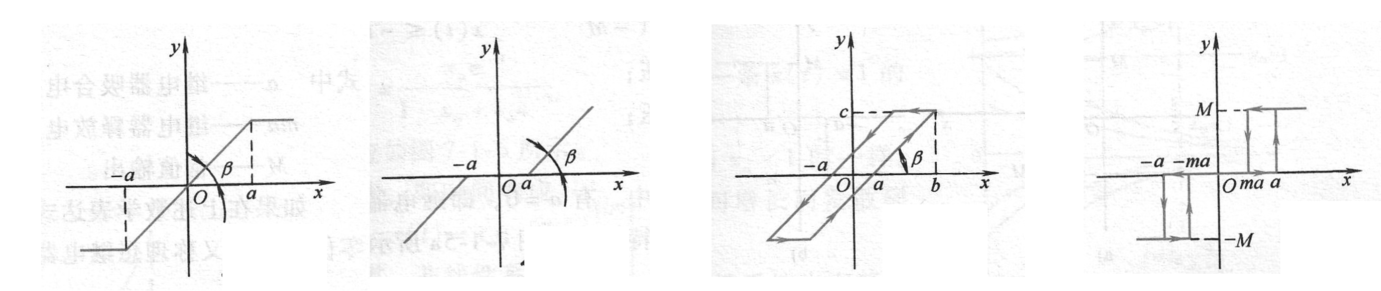
\includegraphics[width=16cm]{典型非线性.png}
                \caption{典型的非线性特性的图像}
            \end{figure}          
    \subsection{相平面法}
        设二阶系统由微分方程$\ddot{x}+f(\dot{x},x)=0$描述，系统的时间解可用以$t$为参变量，用$\dot{x}$和$x$的关系图来表示。
        时间$t$变化时在$x-\dot{x}$平面上绘制出表征系统状态变化过程的轨迹线称作相轨迹，$x-\dot{x}$称为相平面。
        \subsubsection{相轨迹的性质}
            相轨迹的斜率：$\dfrac{\d\dot{x}}{\d x}=-\dfrac{f(x,\dot{x})}{\dot{x}}$

            相轨迹的对称条件：如果$f(x,\dot{x})=f(x,-\dot{x})$，则相轨迹关于$x$轴对称；如果$f(x,\dot{x})=-f(-x,\dot{x})$，则相轨迹关于$\dot{x}$轴对称；
            如果$f(x,\dot{x})=f(-x,-\dot{x})$，则相轨迹关于原点对称。

            相平面图的奇点：同时满足$\dot{x}=0$和$f(x,\dot{x})=0$的点称作奇点。如果一条线每一点都是奇点，则称此直线为奇线。在奇点处相轨迹相交，奇点是相平面的一个平衡点。

            相轨迹通过$x$轴的斜率：除去奇点外，相轨迹和$x$轴垂直相交。

            相轨迹的运动方向：在相平面的上半平面，$\dot{x}>0$，相轨迹运动方向是沿增大的方向即左向右运动；在下半平面，相轨迹运动方向是右向左运动。
        \subsubsection{相轨迹的绘制}
            \begin{itemize}
                \item 解析法：由$\dfrac{\d\dot{x}}{\d x}=-\dfrac{f(x,\dot{x})}{\dot{x}}$积分得到相轨迹方程。
                \item 等倾线法：令$a=-\dfrac{f(x,\dot{x})}{\dot{x}}$，得到一组有同一斜率的点，连接起来得到等倾线，等倾线构成相平面的方向场。
                \item $\delta$法：
                将$\ddot{x}=-f(x,\dot{x},t)$改写成$\ddot{x}+\omega^2x=-f(x,\dot{x},t)+\omega^2x$，使得$\delta(x,\dot{x},t)=\dfrac{-f(x,\dot{x},t)+\omega^2x}{\omega^2}$不太大也不太小。
                取微元时，$\delta$为常量，代入得$\ddot{x}+\omega^2(x-\delta)=0$，整理得相轨迹方程为$\big(\dfrac{\dot{x}}{\omega}\big)^2+(x-\delta)^2=R^2$，即圆弧，将所有圆弧连接得到相轨迹。  
            \end{itemize}        
        \subsubsection{相平面图的分析}
            求运动时间解：(1)根据$\Delta t=\dfrac{\Delta x}{\dot{x}}$求；(2)根据$\displaystyle t=\int\dfrac{1}{\dot{x}}\d x$求；(3)基于$\delta$法圆弧近似得$t\approx\dfrac{\theta}{\omega}$

            \begin{figure}[H]
                \centering
                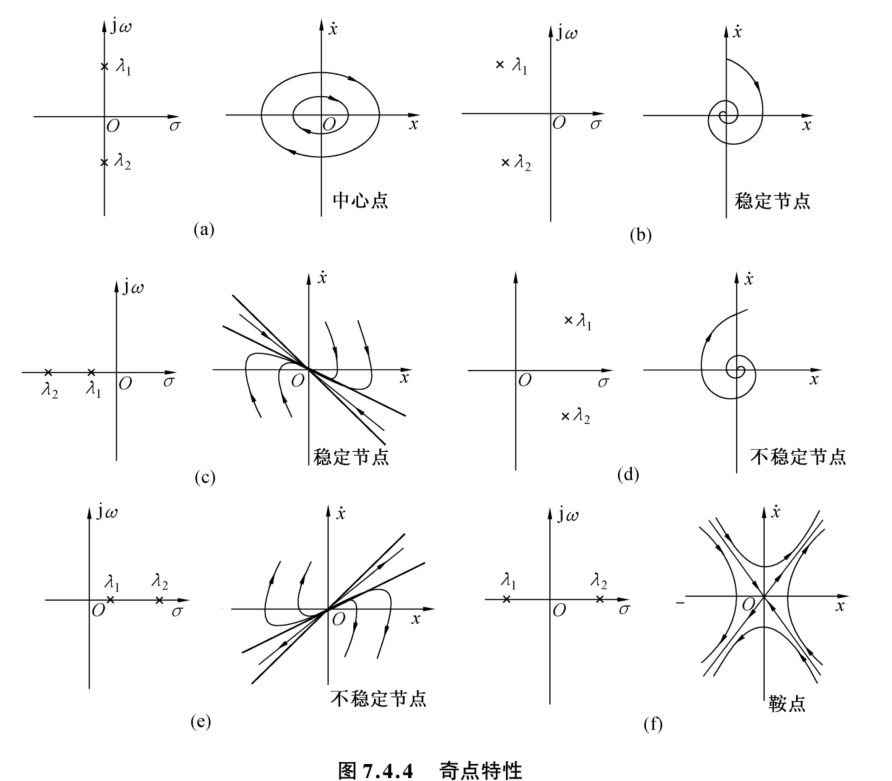
\includegraphics[width=8cm]{线性系统相平面图.png}
                \caption{二阶线性系统的相平面图}
            \end{figure}

            线性化：在奇点附近，Taylor展开系统状态方并取一阶近似得$\begin{cases}\dot{x}_1&=ax_1+bx_2\\\dot{x}_2&=cx_1+dx_2\end{cases}$

            在相平面中，极限环为一条孤立的封闭曲线。
            
            $t\rightarrow\infty$时，在极限环邻域的所有轨迹都收敛于该环，则为稳定极限环，运动是一种稳定的自持振荡。

            $t\rightarrow\infty$时，在极限环内外两侧的所有轨迹都从极限环离开，则为不稳定极限环，极限环内部运动收敛于内部奇点，外部运动发散至无穷远。

            $t\rightarrow\infty$时，在极限环邻域的一些轨迹收敛而一些轨迹离开，则为半稳定极限环。
    \subsection{描述函数法}
        非线性系统可以由线性环节$G(s)$和非线性环节$N(x)$组成。线性输入能展开成高次谐波之和，输出进行傅里叶（Fourier）级数展开，由于低通特性，滤去高次谐波，得到最低次谐波的输出信号。

        输入$e(t)=A\sin\omega t$，对应的输出为$y_1(t)=Y_1\sin(\omega t+\phi_1)$，则描述函数$N(A)=\dfrac{Y_1}{A}\e^{\j\phi_1}$

        系统的传递函数$\varPhi(s)=\dfrac{N(A)G(\j\omega)}{1+N(A)G(\j\omega)}$，特征方程$N(A)G(\j\omega)+1=0$。
        \subsubsection{典型非线性环节的描述函数}
            \begin{itemize}
                \item 饱和特性：$N(A)=\dfrac{2A}{\pi}\big[\arcsin\dfrac{a}{A}+\dfrac{a}{A}\sqrt{1-\big(\dfrac{a}{A}\big)^2}\big],A\geqslant a$
                \item 死区特性：$N(A)=\dfrac{2K}{\pi}\big[\dfrac{\pi}{2}-\arcsin\dfrac{a}{A}-\dfrac{a}{A}\sqrt{1-\big(\dfrac{a}{A}\big)^2}\big],A\geqslant a$
                \item 间隙特性：$N(A)=\dfrac{k}{\pi}\big[\dfrac{\pi}{2}+\arcsin\big(1-\dfrac{2\varepsilon}{A}\big)
                +2\big(1-\dfrac{2\varepsilon}{A}\big)\sqrt{\dfrac{\varepsilon}{A}\big(1-\dfrac{\varepsilon}{A}\big)}\big]
                +\j\dfrac{4k\varepsilon}{\pi A}\big(\dfrac{\varepsilon}{A}-1),A\geqslant\varepsilon$
                \item 具有死区和滞环的继电器特性：
                $N(A)=\dfrac{2M}{\pi A}\big[\sqrt{1-\big(\dfrac{me_0}{A}\big)^2}+\sqrt{1-\big(\dfrac{e_0}{A}\big)^2}\big]+\j\dfrac{2Me_0}{\pi A^2}(m-1),A\geqslant e_0$
            \end{itemize}            
        \subsubsection{稳定性分析}
            系统产生自持振荡的必要条件$1+N(A)G(\j\omega)=0$即$G(\j\omega)=-\dfrac{1}{N(A)}$，因此$-\dfrac{1}{N(A)}$为稳定临界点的轨迹，称作非线性特性的负倒描述函数。

            (1)若$-\dfrac{1}{N(A)}$的曲线始终位于$G(\j\omega)$曲线的左侧，系统稳定，不产生自持振荡；

            (2)若$-\dfrac{1}{N(A)}$的曲线始终位于$G(\j\omega)$曲线的右侧，系统不稳定，不产生自持振荡；

            (3)若$-\dfrac{1}{N(A)}$的曲线与$G(\j\omega)$曲线相交，相交点产生自持振荡，
            若沿幅值$A$增加，$-\dfrac{1}{N(A)}$的曲线进入$G(\j\omega)$曲线内，自持振荡不稳定；
            若沿幅值$A$增加，$-\dfrac{1}{N(A)}$的曲线离开$G(\j\omega)$曲线内，自持振荡稳定。

            \begin{figure}[H]
                \centering
                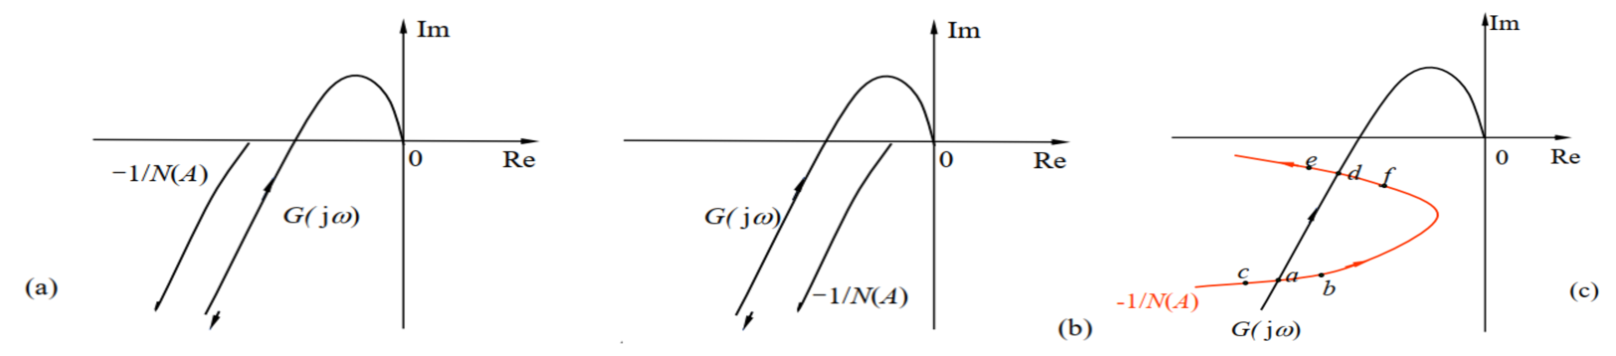
\includegraphics[width=16cm]{描述函数与Nyquist.png}
                \caption{稳定性的三种情况}
            \end{figure}
\end{document}